\documentclass[12pt,a4paper]{article}
\usepackage[a4paper,top=35mm,right=20mm,left=35mm,bottom=20mm]{geometry}
\usepackage[utf8]{inputenc}
\usepackage{amsmath}
\usepackage{amsfonts}
\usepackage{amssymb}
\usepackage{hyperref}
\hypersetup{colorlinks=true}
\hypersetup{pdfborder={0 0 0}}
%\usepackage{tikz}
%\usepackage{pstricks}
\usepackage{graphicx}
\author{Prakash Gautam}
\begin{document}
\begin{titlepage}
		\begin{center}
		\begin{Huge}
			\textbf{Tribhuvan University}\\
			
\includegraphics[scale=1.6]{./Images/logo.png}\\
			Institute of Engineering\\
			Pulchowk Campus\\[1.6cm]		
		\end{Huge}
		\textbf{A\\
		Final Report on\\
		USB Oscilloscope Project}\\[1cm]
		\textbf{Submitted To:}\\
		Department of\\
		Electronics and Computer\\Engineering\\[1.6cm]
	
		\textbf{Submitted By:}\\
		Prajjwal Raj Kandel (068BEX428)\\
		Prakash Gautam (068Bex429)\\
		Sudip Prasai (068BEX442)\\
		Utsav Bhetwal (068BEX447)\\[1.5cm]
		August 26, 2014	
	\end{center}
\end{titlepage}

\pagenumbering{roman}
\vfill

\begin{center}
	\begin{Large}
		\textbf{Approval Sheet}\\[1cm]
	\end{Large}
	\vfill
	TRIBHUVAN UNIVERSITY\\
	INSTITUTE OF ENGINEERING\\
	PULCHOWK CAMPUS\\
	DEPARTMENT OF ELECTRONICS AND COMPUTER ENGINEERING\\
\end{center}
The undersigned certify that they have read, and recommended to the Institute of Engineering for acceptance, a project report entitled \emph{"USB Oscilloscope"}  submitted by Prajjwal Raj Kandel (068BE428), Prakash Gautam (068BEX429), Sudip Prasai(068BEX442) and Utsav Bhetwal(068BEX447), in partial fulfilment of the requirements for the Bachelor’s degree in Electronics and Communication Engineering.


\begin{tabular}{c c}
{}&{}\\
{}&{}\\
------------------------ & ---------------------\\

Supervisor, Dr. Ram Krishna Maharjan \qquad & Supervisor, Dr. Dibakar Raj Pant \\
Associate Professor & Head of Department\\
Department of Electronics & Department of Electronics \\
and Computer Engineering & and Computer Engineering \\
Central Campus & Central Campus\\
Institute of Engineering & Institute of Engineering\\

{}&{}\\
{}&{}\\
---------------------- & -----------------------\\
External Examiner,  Dr.  Surendra  Shrestha & External Examiner,  Mr.  Uttam  Mali\\
Associate  Professor & Associate  Professor\\
Department of Electronics & Department of Electronics \\
and Computer Engineering & and Computer Engineering \\
Central Campus & Central Campus\\
Institute of Engineering & Institute of Engineering\\

\end{tabular}

\vfill
Approved on August 26, 2014

\vfill
\newpage

\begin{flushleft}


\begin{Huge}

A\\
Report on\\
USB Oscilloscope\\[2cm]

\end{Huge}
Copyright $\copyright$ 2014 \textbf{Authors}\\[2cm]

The author has agreed that the Library, Department of Electronics and Computer
Engineering, Pulchowk Campus, Institute of Engineering may make this report freely
available for inspection. Moreover, the author has agreed that permission for
extensive copying of this project report for scholarly purpose may be granted by the
supervisors who supervised the project work recorded herein or, in their absence, by
the Head of the Department wherein the project report was done. It is understood that
the recognition will be given to the author of this report and to the Department of
Electronics and Computer Engineering, Pulchowk Campus, Institute of Engineering
in any use of the material of this project report. Copying or publication or the other
use of this report for financial gain without approval of to the Department of
Electronics and Computer Engineering, Pulchowk Campus, Institute of Engineering
and author’s written permission is prohibited.\\[1cm]
Typeset \LaTeX {} using pdfTeX 3.1415926-2.4-1.40.13\\
(TeX Live 2012/Debian)\\
kpathsea version 6.1.0


\vfill
First printed on August 26, 2014

\end{flushleft}

\newpage
\section*{Preface}
This is a report on USB Oscilloscope, submitted to the department of Electronics and Communication Engineering, Pulcowk Lalitpur. This report primarily describes the project in plain language intended for general reader in mind. 


Our project in the final completed form is intended to general users whose concern is only the output waveform and not on the technical details of the components involved and the software programming. We have tried to avoid the techical details of the software.


The software interface is made simple as possible to allow the general user understand it quickly and be able to use freely in no time. We have tried to make the user interface as close to the actual oscilloscope as possible.


In the very beginning we had plans in mind to make the oscilloscope out of a old CRT TV but after quite a exploration and brain stroming we concluded that we would better be making the oscilloscope based on USB and not on the CRT TV. 


We are especially thankful to Mr.Sumit Bam Shrestha for providing us with ecouragements and invaluable suggestions in the very beginning.


We would also like to thank all our friends, without whose help this project would not have been a success. We would like extend our sincere gratitude and respect to Dr. Diwakar Raj Panta and Dr. Ram Krishna Maharjan--the concerned teachers for handling this minor project of 068BEX. Also we would like to thank the department of Electronics and Computer Engineering, Pulchowk campus for encouraging us to accomplish this project.
\newpage
\tableofcontents

\newpage
\listoffigures

\listoftables
\newpage


\abstract{This is the final report of out Project USB Oscilloscope. After three months of explorations and hard work, we are at a point where we can observe the waveforms of continuous time varying input signals on the PC screen.

First the input analog signal was sampled and the analog to digital conversion was done. Atmega16 microcontroller and the ADC availabe within the same microcontroller is used for this purspose. Then the digital values were sent to the PC via USB following the USB protocol. The program required for microcontorller was written in C++ programming language and was compiled using avr-gcc compiler.

 The digital data was read PC and was converted back to analog values and plotted in graph as a function of time. The software interface required to display the waveform was was built in C++ programmig language using wxWidget API, in our own native style as per the contextual requirement.

Now our system is able to read the input signals. send them to PC. and the PC displays them as a function of time which is exactly the waveform shown by the oscilloscope.\\



\newpage

\pagenumbering{arabic}

\section{Introduction}
One of the most frequent experiments students and researchers would do, working on study of electrical signals is to trace out the waveform of the signal as a function of time. This is what an Oscilloscope does. But the price that is attached with a modern day Oscilloscope of a reasonable performance is beyond reach of many students. \\

The usefulness of an oscilloscope is well known to the students of science and engineering. More often than not while studying various electronics components for learning purpose, students of engineering need to observe the behavioral change of an electrical signal over time. The observed waveform can be analyzed for the properties such as amplitude, frequency, rise time, time interval, distortion and others. For experimenting or being engaged with some projects as well, students need to observe the waveforms of the input signals. Therefore, oscilloscope is very useful device for modern day students \\

In context of countries like Nepal, schools and colleges check their budget twice before even thinking of buying a new oscilloscope, let alone the curious students like us who can't even think of it.\\

But since computers have been vastly cheap and well within the reach of people in general, it makes sense to use the computational power of a computer to do the job of an oscilloscope. Our project is based upon the same idea of making oscilloscope assuming the availability of computer with relative ease than an oscilloscope. \\

Furthermore, parents would rather buy a multipurpose computer rather than an oscilloscope. Additional small aid box beside that computer making it function as an oscilloscope does sound extremely great. \\

Oscilloscopes fall into variety of categories. The biggest distinction is whether they are analogue or digital, but within the digital oscilloscope arena there are ordinary digital oscilloscopes, digital storage oscilloscopes, digital phosphor oscilloscopes, and digital sampling oscilloscopes.

\subsection{Analogue Oscilloscope}
	The analogue oscilloscope of the original type of oscilloscope. As the name implies it uses analogue techniques throughout to create the pattern on the display. Typically they use a cathode ray tube where the voltages on the $x$ and $y$ plats cause a dot on the screen to move. In the horizontal direction this is controlled by the time base, whereas in the vertical direction the deflection is proportional to the signal input. Essentially the signal is amplified and applied to the Y plates of the cathode ray tube using analogue technology

\subsection{Digital Oscilloscope}
	The concept behind the digital oscilloscope is somewhat different to an analogue scope. Rather than processing the signals in an analogue fashion, this type of scope converts the signal into a digital format using an analogue to digital converter and then processes the signals digitally. With digital signal processing hardware and software becoming more powerful, this enables the processing of the signals to be undertaken in a far more flexible manner, and enables many additional features to be included within the scope. Updates and additional functionality can then be made by simply upgrading the software of firmware within the scope.
	
\subsection{USB Oscilloscope} 
	One particular variant this approach that has become very popular what is often termed the USB oscilloscope the name implies, the USB oscilloscope interface with a PC using the USB connector. This provides an effective interface for communication between the two elements. While this type of approach may not be suitable in many specific and critical applications, it is ideal for many others where general purpose PC can be used. 





\section{Objectives}
	As a part of syllabus of IOE, students of III${}^{rd}$ yr II${}^{nd}$ part are required to carry out a mini project. This project of ours is primarily intended for the fulfillment of the same. But we are committed to make this project not \emph{just another project}, we are expecting some real usefulness beside completing the requirement together with learning basic hardware electronics coupled with software interface.\\

	We hope to learn a great deal of electronics on the application level.\\

	Some of the objectives can be listed as:\\
	
	\begin{enumerate}
		\item To fulfill the course requirement.
		\item To learn software and hardware integration on real scale
		\item To learn the micro-controller programming
		\item To learn to develop the hardware circuitry through PCB technique
		\item To create easily affordable oscilloscope for students.
	\end{enumerate}

	\section{Hardware Selection and Software}
		Different hardware components used in the project are described in brief in the following section. Micro-controller is the primary hardware used and the major hardware is the display unit of computer.
	\subsection{Microcontroller}
		We have used ATMEGA16 as the Micro-controller. It has a built in ADC of 10-bit resolution and can run at a clock frequency 16MHz which is sufficient for our requirement of the ADC conversion rate.

		\begin{figure}[h]	
			\centering
			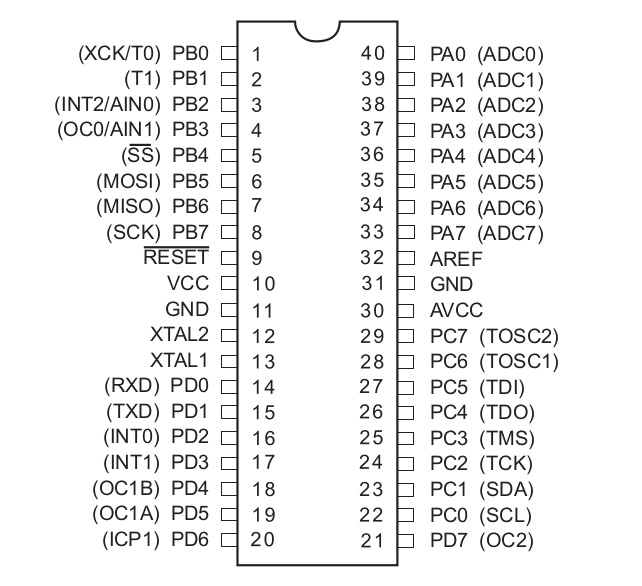
\includegraphics[scale=.35]{Images/Atmega16PinOut.png}
			\caption{Atmega16 Pinout}
			\label{fig:PinOut}
		\end{figure}

Also it provides 16KB flash memory which is sufficient for our project.



\subsection{Voltage attenuator}
Since the input voltage of the Microcontroller is just 5V, and our oscilloscope needed to convert wider ranges of voltages into the range 0-5V, for this we needed voltage attenuator. We have decided to use instrumentation amplifier to regulate voltage to that level. The schematic circuit for the voltage attenuator is:
\begin{figure}[hbtp]
	\centering
	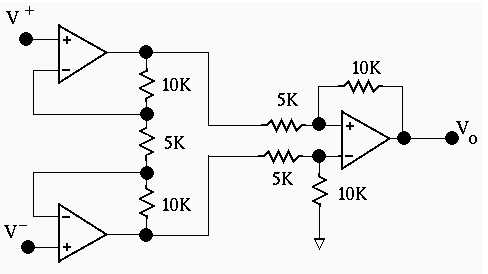
\includegraphics[scale=.4]{./Images/Amplifier.png}
	\caption{Instrumentation Amplifier}
\end{figure}


\subsection{Program Compiler and Up-loader}	
We have even made our own programming software interface. This utilizes the \emph{avr-gcc} compiler and uses avrdude to interface the programmer and the software interface. This can be used to upload program to various variants of atmega microcontroller.\\ This can be used to program other microcontrollers of the AVR family. One snapshot of the program compiler is given in Figure \ref{fig:Programmer}.



\begin{figure}[hbtp]
\centering
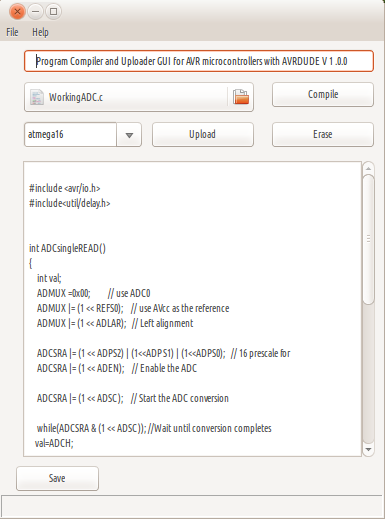
\includegraphics[scale=.5]{Images/AvrGUI.png}
\caption{Programmer Software Interface}
\label{fig:Programmer}
\end{figure}

This too is made in C++ programming language with wxWidget and can easily be extended to write program for other microcontrollers too. 

\section{System Block Diagram}
	The system block diagram of the system overview is given in Figure\ref{fig:BlockDiagram}. Various stages of input processing and output are shown in this figure.
	\begin{figure}[hbtp]
		\centering
		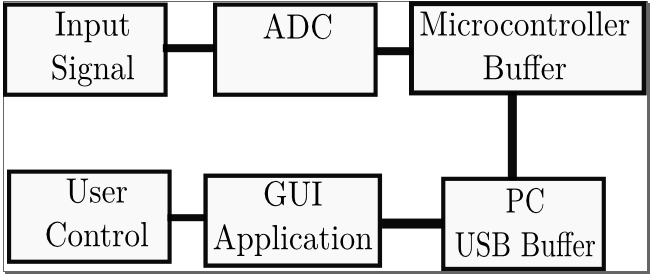
\includegraphics[scale=.6]{Images/BlockDiagram.png}
		\caption{Block Diagram}
		\label{fig:BlockDiagram}
	\end{figure}


\section{Circuit Schematics}
The usb oscilloscope circuit is a fairly simple circuit with not complications and difficulty in understanding. It just has the interface to input the signal and has necessary mechanisms to convert the signals and send to PC via USB cable.

\begin{figure}[hbtp]
	\centering
	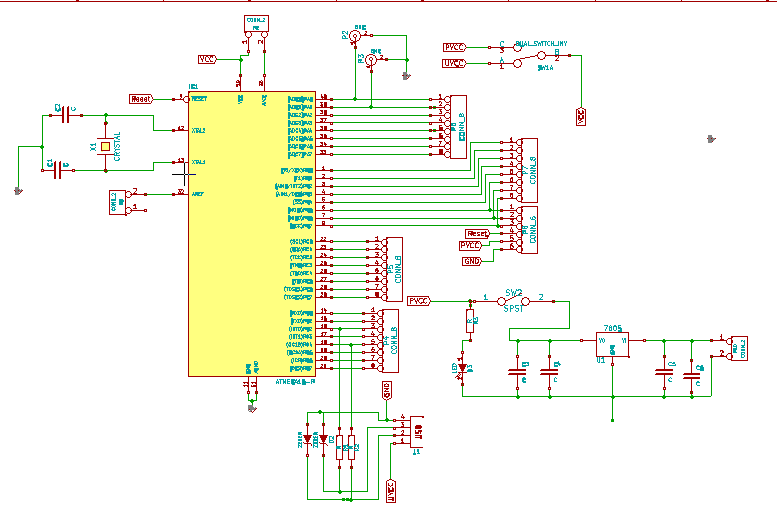
\includegraphics[scale=.4]{Images/CircuitTwoD.png}
	\caption{Circuit schematics }
\end{figure}

\section{Basic operation}
At first the analog input signals are fed to an ADC to convert them to digital values that a computer can compute. For this very project, the built-in ADC available in the microcontroller Atmega16 is used. Among four ports of Atmega16, Port A provides the features of ADC.

\subsection{Inputting a signal}

To use the oscilloscope, desired signal should be input  to the input connector of the oscilloscope. Coaxial connectors are used for inputting the signals. Since this is a dual channel oscilloscope, two connectors are used. BNC connectors are the first choice to reduce noise and safely transfer the signal from source to the Oscilloscope device.
Basic operation: 


\subsection{Analog to Digital Conversion}
The ATmega16 features a 10-bit successive approximation ADC. The ADC is connected to an
8-channel Analog Multiplexer which allows 8 single-ended voltage inputs constructed from the
pins of Port A. The single-ended voltage inputs refer to 0V (GND). But for our purpose we have used only 8 bit resolution of the ADC.

The ADC contains a Sample and Hold circuit which ensures that the input voltage to the ADC is
held at a constant level during conversion.

The ADC is fairly fast  
\begin{table}[ht]
	\centering
	\begin{tabular}{|l|c|c|}
		\hline 
		Condition & Sample Hold Cycles & Comversion Time \\ 
		\hline 
		First Conversion & 13.5 & 13 \\ 
		\hline 
		Normol Conversion & 1.5 & 13 \\ 
		\hline 
		Auto Triggered conversions & 2 & 13.5 \\ 
		\hline 
		Normal Conversions Differential & 1.5/2.5 & 13/14 \\ 
		\hline 
	\end{tabular}
	
	\caption{ADC Conversion Time} 
	\label{tab:ADCCnvTime}
\end{table}
In Table \ref{tab:ADCCnvTime} we can see the conversion time of the Atmega16
The ADC converts an analog input voltage to a 10-bit digital value through successive approximation. The minimum value represents GND and the maximum value represents the voltage on the AREF pin minus 1 LSB. Optionally, AVCC or an internal 2.56V reference voltage may be connected to the AREF pin by writing to the REFSn bits in the ADMUX Register. The internal voltage reference may thus be decoupled by an external capacitor at the AREF pin to improve noise immunity.\footnote{This is taken form Atmega16 datasheet}

\subsection{Sensing}
First the input signal will be converted into Digital signal with a high speed ADC. If the frequency of input signal is $f$ and $n$ samples are taken per cycle of the signal then the frequency of sampling will be:
\begin{equation}
	\textit{Sampling Frequency}= f*n
\end{equation}
Owing to Nyquist criterion the value of $n$  should be greater than $2$ but this will not suffice to generate smooth signal so we will need $n\geq 100$.\\

If we restrict ourselves with the input frequency of the order of hundred of kilo hertz then. The sampling frequency should be around
\begin{eqnarray*}
 \textit{Sampling Frequency}&=&100K*100\\
 &=& 10MHz\\
\end{eqnarray*}

So we would require ADC with the output time less than $10^{-7}s$. \\

Also thre is a limitaion of number of bits of output bits of ADC. To minimize the cost and optimize the system performance we would use a $10$bit ADC. Now the rate of generation of data is given bye the relation \\
\begin{eqnarray*}
\textit{Data Rate}&=&\textit{no. of bits}*\textit{Sampling Frequency}\\
&=& \textsl{no.of bits}*f*n\\
& \approx &10\textsl{bits}*100\textsl{K}*100\\
&=&100\textsl{Mbps}
\end{eqnarray*}

Since the speed of USB $2.0$ is $480$Mbps in full speed mode, this data rate can be handled by USB data communication.\\



\subsection{Communication with PC}
The communication with PC has two distinct parts
\begin{enumerate}
	\item Firmware on Device
	\item Host Driver Software on PC
\end{enumerate}
\subsection{Firmware}
To make the interface to communicate with pc we have used VUSB library available at \url{http://obdev.net}. This library helps to communicate data between PC and the microcontroller. Our device falls in HID class device. The firmware does the necessary tasks required for preparation of data from ADC and putting it in device buffer. And send data to the PC following the USB protocol.

Since the ADC available in the microcontroller is used, the outputs of ADC, i.e. digital values are stored in a registers of the microcontroller itself. Now the digital values from a register of Atmega16 are continuously fed to the PC through the USB cable following the USB protocols. 

\subsection{Host Software}
Once the data is received in the computer, the task remaining is to trace out the values on PC screen. For plotting this data into the screen as a function of time, we have prepared a graph plotting software ourselves, which plots the values received at the PC through USB port into the display of the PC making the waveform of the input signals visible. 

Host software again makes use of libusb library to make proper communication with the firmware on the device. A channel is formed between the host software and device through the USB connection.


The software interfaces are made in C++ programming language and compiled for Linux Operating system. But the programms are made platform independent and can be easily compiled for other operating systems with just minor changes

\subsection{Graph Plotter}
We have made a graph plotter in C++ programming language with \textit{WxWidget 3.0.0} library. This plotter will be used to show the graphical representation of the waveform. The interface looks like. It is yet to be improved to give a look and feel like a real oscilloscope interface but nonetheless it servers the basic purpose of user control and displaying.
\begin{figure}[hbtp]
	\centering
	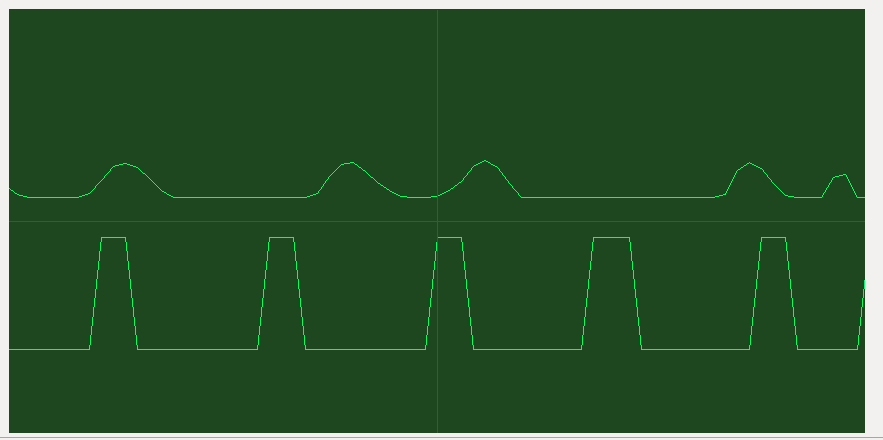
\includegraphics[scale=.4]{Images/DualChannel.png}
	\caption{Oscilloscope display interface}
\end{figure}
Since it is a dual channel oscilloscope features like selection of channel is inherently required and is made but other fancy looks are still to be added. At the moment we can vary the frequency scale and amplitude scale with the obvious requirement of hold.


\subsubsection{The Trace}
The trace is one of the most basic operations of oscilloscope. The oscilloscope draws a trace, which is a horizontal line across the screen. The time base control determines how quickly the trace is drawn. When the voltage becomes negative or positive, the viewer displays a correspondingly positive or negative jump in the trace on screen.

\subsubsection{Vertical and Horizontal Sensitivity control}


These controls allow the user to determine the sensitivity, both horizontally and vertically. To accommodate a wide range of input amplitudes, vertical control selects the calibrated sensitivity of the vertical deflection. Similarly horizontal control is used for viewing the signals with wide range of frequencies with relative ease.

\subsubsection{Hold}
For high frequency signals, it is not possible to find out the signal properties like amplitude and phase if the signal waveform just moves on the PC screen rapidly. For these analyses, sometimes it is necessary to hold the output on the screen.  This control allows the user to hold the screen output for such analyses.


\section{Outputs}
After we completed our project we have tested our oscilloscope for various input signals and observed its output waveform. For some of the input signals the following output waveforms were obsesrved.

\begin{description}
	\item[Square Wave] For testing periodic signal we produced square wave from a timer circuit. And a very good wave structure with clear rise and fall time was observed.
	\begin{figure}[hpbt]
		\centering
		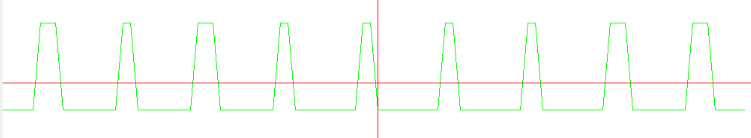
\includegraphics[scale=.5]{./Images/OutputOne.png}
		\caption{Square Wave}
		\label{fig:SquareWave}
\end{figure}				
\end{description}

%%LaTeX with PSTricks extensions
%%Creator: inkscape 0.48.4
%%Please note this file requires PSTricks extensions
\psset{xunit=.5pt,yunit=.5pt,runit=.5pt}
\begin{pspicture}(459.7651062,192.74983215)
{
\newrgbcolor{curcolor}{0.97647059 0.97647059 0.97647059}
\pscustom[linestyle=none,fillstyle=solid,fillcolor=curcolor]
{
\newpath
\moveto(1.48111734,190.26871836)
\lineto(116.14112864,190.26871836)
\lineto(116.14112864,125.90967143)
\lineto(1.48111734,125.90967143)
\closepath
}
}
{
\newrgbcolor{curcolor}{0 0 0}
\pscustom[linewidth=2.9622252,linecolor=curcolor]
{
\newpath
\moveto(1.48111734,190.26871836)
\lineto(116.14112864,190.26871836)
\lineto(116.14112864,125.90967143)
\lineto(1.48111734,125.90967143)
\closepath
}
}
{
\newrgbcolor{curcolor}{0 0 0}
\pscustom[linestyle=none,fillstyle=solid,fillcolor=curcolor]
{
\newpath
\moveto(44.38943232,168.22807981)
\lineto(44.38943232,169.00262039)
\lineto(43.80503666,169.00262039)
\curveto(42.02937468,169.00262039)(41.96194263,169.27745827)(41.96194263,170.17692384)
\lineto(41.96194263,183.3441136)
\curveto(41.96194263,184.24357918)(42.02937468,184.51841706)(43.80503666,184.51841706)
\lineto(44.38943232,184.51841706)
\lineto(44.38943232,185.29295763)
\curveto(43.60274664,185.21800217)(41.82708124,185.21800209)(40.97296535,185.21800209)
\curveto(40.09637273,185.21800209)(38.32070731,185.21800217)(37.53402162,185.29295763)
\lineto(37.53402162,184.51841706)
\lineto(38.11841729,184.51841706)
\curveto(39.89407927,184.51841706)(39.96151131,184.24357918)(39.96151131,183.3441136)
\lineto(39.96151131,170.17692384)
\curveto(39.96151131,169.27745827)(39.89407927,169.00262039)(38.11841729,169.00262039)
\lineto(37.53402162,169.00262039)
\lineto(37.53402162,168.22807981)
\curveto(38.32070731,168.30303528)(40.09637271,168.30303535)(40.9504886,168.30303535)
\curveto(41.82708122,168.30303535)(43.60274664,168.30303528)(44.38943232,168.22807981)
}
}
{
\newrgbcolor{curcolor}{0 0 0}
\pscustom[linestyle=none,fillstyle=solid,fillcolor=curcolor]
{
\newpath
\moveto(57.0512213,168.22807981)
\lineto(57.0512213,169.00262039)
\curveto(55.88243114,169.00262039)(55.32051103,169.00262114)(55.2980343,169.75217578)
\lineto(55.2980343,174.52434513)
\curveto(55.2980343,176.67306844)(55.2980336,177.44761207)(54.60125485,178.34707764)
\curveto(54.28658058,178.77182527)(53.544846,179.27152929)(52.24119543,179.27152929)
\curveto(50.60039385,179.27152929)(49.54398403,178.19716501)(48.91463548,176.64808541)
\lineto(48.91463548,179.27152929)
\lineto(45.74541283,178.99669232)
\lineto(45.74541283,178.22215174)
\curveto(47.31878421,178.22215174)(47.49859983,178.04725426)(47.49859983,176.82298167)
\lineto(47.49859983,170.12695348)
\curveto(47.49859983,169.00262151)(47.25135401,169.00262039)(45.74541283,169.00262039)
\lineto(45.74541283,168.22807981)
\lineto(48.28528631,168.30303535)
\lineto(50.80268302,168.22807981)
\lineto(50.80268302,169.00262039)
\curveto(49.29674185,169.00262039)(49.04949602,169.00262151)(49.04949602,170.12695348)
\lineto(49.04949602,174.72422657)
\curveto(49.04949602,177.32268267)(50.64534717,178.72185534)(52.08385814,178.72185534)
\curveto(53.49989237,178.72185534)(53.74713811,177.3726542)(53.74713811,175.94850038)
\lineto(53.74713811,170.12695348)
\curveto(53.74713811,169.00262151)(53.49989228,169.00262039)(51.99395111,169.00262039)
\lineto(51.99395111,168.22807981)
\lineto(54.53382458,168.30303535)
\lineto(57.0512213,168.22807981)
}
}
{
\newrgbcolor{curcolor}{0 0 0}
\pscustom[linestyle=none,fillstyle=solid,fillcolor=curcolor]
{
\newpath
\moveto(69.24802259,173.62487866)
\curveto(69.24802259,176.79799332)(67.0677747,179.27152929)(64.5503805,179.27152929)
\curveto(62.79719526,179.27152929)(61.85316928,178.17218083)(61.40363461,177.62250743)
\lineto(61.40363461,179.27152929)
\lineto(58.16698169,178.99669232)
\lineto(58.16698169,178.22215174)
\curveto(59.76282979,178.22215174)(59.92016868,178.07223956)(59.92016868,176.97289275)
\lineto(59.92016868,165.2798286)
\curveto(59.92016868,164.15549663)(59.67292286,164.1554955)(58.16698169,164.1554955)
\lineto(58.16698169,163.38095493)
\lineto(60.6843784,163.45591047)
\lineto(63.22425187,163.38095493)
\lineto(63.22425187,164.1554955)
\curveto(61.7183107,164.1554955)(61.47106488,164.15549663)(61.47106488,165.2798286)
\lineto(61.47106488,169.47733881)
\lineto(61.47106488,169.70220542)
\curveto(61.58344855,169.30244295)(62.52747413,167.95324284)(64.23570591,167.95324284)
\curveto(66.91043725,167.95324284)(69.24802259,170.40179368)(69.24802259,173.62487866)
\moveto(67.38245181,173.62487866)
\curveto(67.38245181,170.60167492)(65.8090772,168.50291679)(64.14579889,168.50291679)
\curveto(63.24672953,168.50291679)(62.39261128,169.00262141)(61.78573947,170.02701276)
\curveto(61.47106519,170.55170101)(61.47106488,170.57668722)(61.47106488,171.07639031)
\lineto(61.47106488,176.64808541)
\curveto(62.12289016,177.92232831)(63.22425302,178.6468998)(64.37056645,178.6468998)
\curveto(66.01136803,178.6468998)(67.38245181,176.44820115)(67.38245181,173.62487866)
}
}
{
\newrgbcolor{curcolor}{0 0 0}
\pscustom[linestyle=none,fillstyle=solid,fillcolor=curcolor]
{
\newpath
\moveto(82.07417215,168.22807981)
\lineto(82.07417215,169.00262039)
\curveto(80.50080078,169.00262039)(80.32098515,169.17751787)(80.32098515,170.40179046)
\lineto(80.32098515,179.27152929)
\lineto(77.01690196,178.99669232)
\lineto(77.01690196,178.22215174)
\curveto(78.59027334,178.22215174)(78.77008896,178.04725426)(78.77008896,176.82298167)
\lineto(78.77008896,172.37561966)
\curveto(78.77008896,170.20191119)(77.69120301,168.50291679)(76.05040144,168.50291679)
\curveto(74.16235579,168.50291679)(74.07244687,169.67722154)(74.07244687,170.97644959)
\lineto(74.07244687,179.27152929)
\lineto(70.76836369,178.99669232)
\lineto(70.76836369,178.22215174)
\curveto(72.52154893,178.22215174)(72.52155068,178.14719398)(72.52155068,175.9235152)
\lineto(72.52155068,172.17573823)
\curveto(72.52155068,170.22689615)(72.5215541,167.95324284)(75.93801766,167.95324284)
\curveto(77.19671475,167.95324284)(78.18569395,168.65282942)(78.83751923,170.20190902)
\lineto(78.83751923,167.95324284)
\lineto(82.07417215,168.22807981)
}
}
{
\newrgbcolor{curcolor}{0 0 0}
\pscustom[linestyle=none,fillstyle=solid,fillcolor=curcolor]
{
\newpath
\moveto(90.02286919,171.32624211)
\lineto(90.02286919,172.75039736)
\lineto(89.46095028,172.75039736)
\lineto(89.46095028,171.37621247)
\curveto(89.46095028,169.52731101)(88.78664676,168.57787233)(87.95500761,168.57787233)
\curveto(86.44906643,168.57787233)(86.44906493,170.85152412)(86.44906493,171.27627175)
\lineto(86.44906493,178.22215174)
\lineto(89.66324109,178.22215174)
\lineto(89.66324109,178.99669232)
\lineto(86.44906493,178.99669232)
\lineto(86.44906493,183.5939654)
\lineto(85.88714602,183.5939654)
\curveto(85.86466928,181.54518271)(85.19036437,178.87176632)(82.98764444,178.7718257)
\lineto(82.98764444,178.22215174)
\lineto(84.89816874,178.22215174)
\lineto(84.89816874,171.32624211)
\curveto(84.89816874,168.25306807)(86.98850789,167.95324284)(87.79767031,167.95324284)
\curveto(89.39351842,167.95324284)(90.02286919,169.7271922)(90.02286919,171.32624211)
}
}
{
\newrgbcolor{curcolor}{0 0 0}
\pscustom[linestyle=none,fillstyle=solid,fillcolor=curcolor]
{
}
}
{
\newrgbcolor{curcolor}{0 0 0}
\pscustom[linestyle=none,fillstyle=solid,fillcolor=curcolor]
{
\newpath
\moveto(45.33292929,141.64384849)
\curveto(45.33292929,144.14236397)(43.84946148,146.19115171)(41.96141583,146.69085481)
\lineto(39.08439102,147.46539539)
\curveto(37.69083351,147.84017271)(36.81423862,149.18937424)(36.81423862,150.63851322)
\curveto(36.81423862,152.38747406)(38.02798522,153.91157178)(39.78117046,153.91157178)
\curveto(43.53478503,153.91157178)(44.02927756,149.81400116)(44.16413796,148.6896692)
\curveto(44.1866147,148.53975827)(44.18661496,148.38984704)(44.43385904,148.38984704)
\curveto(44.72605658,148.38984704)(44.72605687,148.51477341)(44.72605687,148.98949135)
\lineto(44.72605687,154.0115125)
\curveto(44.72605687,154.43626013)(44.72605662,154.61115681)(44.47881255,154.61115681)
\curveto(44.32147541,154.61115681)(44.29899834,154.58617133)(44.1416612,154.28634948)
\lineto(43.35497473,152.86219423)
\curveto(42.68067271,153.58676372)(41.75912303,154.61115681)(39.75869371,154.61115681)
\curveto(37.26377624,154.61115681)(35.37572621,152.41245834)(35.37572621,149.76403193)
\curveto(35.37572621,147.69026408)(36.56699605,145.8663432)(38.3201813,145.19174402)
\curveto(38.56742537,145.0918034)(39.71374177,144.79198072)(41.28711314,144.36723309)
\curveto(41.89398496,144.192337)(42.56828889,144.01743965)(43.19763744,143.09298892)
\curveto(43.66964885,142.44337489)(43.89441688,141.61886248)(43.89441688,140.79435237)
\curveto(43.89441688,139.02040638)(42.77057718,137.22147166)(40.88253153,137.22147166)
\curveto(40.23070624,137.22147166)(38.52247092,137.34639878)(37.33120402,138.57067137)
\curveto(36.02755345,139.91986973)(35.96012186,141.51892349)(35.93764512,142.41838906)
\curveto(35.91516839,142.66824061)(35.73535425,142.66824086)(35.66792404,142.66824086)
\curveto(35.3757265,142.66824086)(35.37572621,142.49334415)(35.37572621,142.04361136)
\lineto(35.37572621,137.0465754)
\curveto(35.37572621,136.62182777)(35.37572646,136.44693109)(35.62297053,136.44693109)
\curveto(35.78030767,136.44693109)(35.80278474,136.49690172)(35.96012188,136.77173842)
\curveto(35.96012188,136.77173842)(36.02755289,136.87168047)(36.76928511,138.19589367)
\curveto(37.46606386,137.34639841)(38.90457897,136.44693109)(40.90500828,136.44693109)
\curveto(43.53478615,136.44693109)(45.33292929,138.89548146)(45.33292929,141.64384849)
}
}
{
\newrgbcolor{curcolor}{0 0 0}
\pscustom[linestyle=none,fillstyle=solid,fillcolor=curcolor]
{
\newpath
\moveto(52.18026256,136.99660504)
\lineto(52.18026256,137.77114562)
\curveto(50.69679812,137.77114562)(50.60688961,137.89607249)(50.60688961,138.87049353)
\lineto(50.60688961,148.04005452)
\lineto(47.46014372,147.76521754)
\lineto(47.46014372,146.99067697)
\curveto(48.92113142,146.99067697)(49.12342369,146.84076467)(49.12342369,145.61649208)
\lineto(49.12342369,138.89547871)
\curveto(49.12342369,137.77114674)(48.87617787,137.77114562)(47.37023669,137.77114562)
\lineto(47.37023669,136.99660504)
\lineto(49.8426799,137.07156058)
\curveto(50.62936558,137.07156058)(51.41605361,137.0215902)(52.18026256,136.99660504)
\moveto(50.94404096,152.08765365)
\curveto(50.94404096,152.76225283)(50.42707489,153.41186818)(49.75277287,153.41186818)
\curveto(48.98856392,153.41186818)(48.53902803,152.71228252)(48.53902803,152.08765365)
\curveto(48.53902803,151.41305447)(49.0559941,150.76343912)(49.73029611,150.76343912)
\curveto(50.49450507,150.76343912)(50.94404096,151.46302478)(50.94404096,152.08765365)
}
}
{
\newrgbcolor{curcolor}{0 0 0}
\pscustom[linestyle=none,fillstyle=solid,fillcolor=curcolor]
{
\newpath
\moveto(63.7635177,147.09061769)
\curveto(63.7635177,147.51536532)(63.49379575,148.3148915)(62.61720313,148.3148915)
\curveto(62.16766845,148.3148915)(61.17868977,148.1649794)(60.23466695,147.14058805)
\curveto(59.29064413,147.96509816)(58.34661892,148.04005452)(57.85213077,148.04005452)
\curveto(55.76179452,148.04005452)(54.21089624,146.31607519)(54.21089624,144.39221827)
\curveto(54.21089624,143.29287146)(54.70538544,142.343433)(55.26730379,141.81874475)
\curveto(54.97510625,141.44396742)(54.57052434,140.61945524)(54.57052434,139.74497482)
\curveto(54.57052434,138.97043502)(54.86272287,138.02099691)(55.55950162,137.52129382)
\curveto(54.21089759,137.09654619)(53.49164003,136.02218203)(53.49164003,135.02277584)
\curveto(53.49164003,133.22384469)(55.71684166,131.849658)(58.4590032,131.849658)
\curveto(61.1112578,131.849658)(63.44884311,133.12390412)(63.44884311,135.0727462)
\curveto(63.44884311,135.94722661)(63.13416738,137.22147236)(61.98785395,137.92105669)
\curveto(60.79658705,138.62064103)(59.49293262,138.62064173)(58.12185185,138.62064173)
\curveto(57.5599335,138.62064173)(56.59343226,138.62064175)(56.43609512,138.64562691)
\curveto(55.71683963,138.74556753)(55.24482703,139.520109)(55.24482703,140.31963396)
\curveto(55.24482703,140.41957458)(55.24482741,140.99423431)(55.62693189,141.49393741)
\curveto(56.50352451,140.79435307)(57.42507283,140.71939683)(57.85213077,140.71939683)
\curveto(59.94246703,140.71939683)(61.49336531,142.44337617)(61.49336531,144.36723309)
\curveto(61.49336531,145.29168382)(61.13373664,146.21613697)(60.5718183,146.79079553)
\curveto(61.38098072,147.64029079)(62.19014516,147.76521754)(62.59472637,147.76521754)
\curveto(62.59472637,147.76521754)(62.75206373,147.76521752)(62.81949394,147.74023236)
\curveto(62.57224986,147.64029174)(62.45986583,147.36545437)(62.45986583,147.06563251)
\curveto(62.45986583,146.64088488)(62.75206403,146.34106229)(63.11169177,146.34106229)
\curveto(63.33645911,146.34106229)(63.7635177,146.51595913)(63.7635177,147.09061769)
\moveto(59.80760858,144.39221827)
\curveto(59.80760858,143.71761909)(59.78513149,142.91809203)(59.44798048,142.29346316)
\curveto(59.26816661,141.99364131)(58.75120013,141.29405597)(57.85213077,141.29405597)
\curveto(55.89665492,141.29405597)(55.89665297,143.79257453)(55.89665297,144.36723309)
\curveto(55.89665297,145.04183227)(55.91913006,145.84135932)(56.25628107,146.46598819)
\curveto(56.43609494,146.76581005)(56.95306142,147.46539539)(57.85213077,147.46539539)
\curveto(59.80760662,147.46539539)(59.80760858,144.96687683)(59.80760858,144.39221827)
\moveto(62.28005178,135.02277584)
\curveto(62.28005178,133.67357747)(60.68419988,132.42431713)(58.48147995,132.42431713)
\curveto(56.21132983,132.42431713)(54.66043136,133.69856263)(54.66043136,135.02277584)
\curveto(54.66043136,136.17209296)(55.5145491,137.09654584)(56.50352539,137.1715013)
\lineto(57.82965402,137.1715013)
\curveto(59.76265313,137.1715013)(62.28005178,137.17149915)(62.28005178,135.02277584)
}
}
{
\newrgbcolor{curcolor}{0 0 0}
\pscustom[linestyle=none,fillstyle=solid,fillcolor=curcolor]
{
\newpath
\moveto(76.12573462,136.99660504)
\lineto(76.12573462,137.77114562)
\curveto(74.95694446,137.77114562)(74.39502436,137.77114637)(74.37254763,138.52070101)
\lineto(74.37254763,143.29287036)
\curveto(74.37254763,145.44159367)(74.37254693,146.21613729)(73.67576818,147.11560287)
\curveto(73.3610939,147.5403505)(72.61935932,148.04005452)(71.31570876,148.04005452)
\curveto(69.67490718,148.04005452)(68.61849736,146.96569024)(67.98914881,145.41661064)
\lineto(67.98914881,148.04005452)
\lineto(64.81992616,147.76521754)
\lineto(64.81992616,146.99067697)
\curveto(66.39329753,146.99067697)(66.57311316,146.81577949)(66.57311316,145.5915069)
\lineto(66.57311316,138.89547871)
\curveto(66.57311316,137.77114674)(66.32586733,137.77114562)(64.81992616,137.77114562)
\lineto(64.81992616,136.99660504)
\lineto(67.35979963,137.07156058)
\lineto(69.87719635,136.99660504)
\lineto(69.87719635,137.77114562)
\curveto(68.37125517,137.77114562)(68.12400935,137.77114674)(68.12400935,138.89547871)
\lineto(68.12400935,143.49275179)
\curveto(68.12400935,146.0912079)(69.71986049,147.49038057)(71.15837146,147.49038057)
\curveto(72.5744057,147.49038057)(72.82165143,146.14117943)(72.82165143,144.71702561)
\lineto(72.82165143,138.89547871)
\curveto(72.82165143,137.77114674)(72.57440561,137.77114562)(71.06846444,137.77114562)
\lineto(71.06846444,136.99660504)
\lineto(73.60833791,137.07156058)
\lineto(76.12573462,136.99660504)
}
}
{
\newrgbcolor{curcolor}{0 0 0}
\pscustom[linestyle=none,fillstyle=solid,fillcolor=curcolor]
{
\newpath
\moveto(87.46842007,139.22028605)
\lineto(87.46842007,140.61945612)
\lineto(86.90650116,140.61945612)
\lineto(86.90650116,139.22028605)
\curveto(86.90650116,137.77114707)(86.34458201,137.62123454)(86.09733793,137.62123454)
\curveto(85.35560572,137.62123454)(85.26569795,138.74556775)(85.26569795,138.87049353)
\lineto(85.26569795,143.86752949)
\curveto(85.26569795,144.91690599)(85.26569714,145.89132998)(84.45653472,146.81578071)
\curveto(83.5799421,147.79020175)(82.45610232,148.1899656)(81.37721909,148.1899656)
\curveto(79.53412691,148.1899656)(77.98322888,147.0156605)(77.98322888,145.36664028)
\curveto(77.98322888,144.61708564)(78.43276459,144.19233683)(79.01715967,144.19233683)
\curveto(79.64650822,144.19233683)(80.05109046,144.69204108)(80.05109046,145.3416551)
\curveto(80.05109046,145.64147696)(79.93870565,146.46598822)(78.90477589,146.49097337)
\curveto(79.5116477,147.36545379)(80.61301009,147.64029164)(81.33226558,147.64029164)
\curveto(82.43362554,147.64029164)(83.71480176,146.66586741)(83.71480176,144.44218863)
\lineto(83.71480176,143.51773697)
\curveto(82.56848833,143.44278151)(80.99511282,143.36782515)(79.57907858,142.6182705)
\curveto(77.89332354,141.76877524)(77.33140294,140.46954394)(77.33140294,139.37019712)
\curveto(77.33140294,137.34639958)(79.51164973,136.72176806)(80.92768396,136.72176806)
\curveto(82.4111484,136.72176806)(83.44508111,137.72117643)(83.87213905,138.89547871)
\curveto(83.96204599,137.89607251)(84.56891956,136.84669396)(85.62532605,136.84669396)
\curveto(86.09733746,136.84669396)(87.46842007,137.1964885)(87.46842007,139.22028605)
\moveto(83.71480176,140.49453022)
\curveto(83.71480176,138.12094051)(82.09647429,137.27144202)(81.08502126,137.27144202)
\curveto(79.9836613,137.27144202)(79.06211318,138.14592456)(79.06211318,139.3951823)
\curveto(79.06211318,140.76936582)(80.00614066,142.84313727)(83.71480176,142.9930482)
\lineto(83.71480176,140.49453022)
}
}
{
\newrgbcolor{curcolor}{0 0 0}
\pscustom[linestyle=none,fillstyle=solid,fillcolor=curcolor]
{
\newpath
\moveto(93.58209691,136.99660504)
\lineto(93.58209691,137.77114562)
\curveto(92.07615574,137.77114562)(91.82890991,137.77114674)(91.82890991,138.89547871)
\lineto(91.82890991,154.33631984)
\lineto(88.59225699,154.06148286)
\lineto(88.59225699,153.28694228)
\curveto(90.16562836,153.28694228)(90.34544399,153.1120448)(90.34544399,151.88777221)
\lineto(90.34544399,138.89547871)
\curveto(90.34544399,137.77114674)(90.09819816,137.77114562)(88.59225699,137.77114562)
\lineto(88.59225699,136.99660504)
\lineto(91.08717695,137.07156058)
\lineto(93.58209691,136.99660504)
}
}
{
\newrgbcolor{curcolor}{0.97647059 0.97647059 0.97647059}
\pscustom[linestyle=none,fillstyle=solid,fillcolor=curcolor]
{
\newpath
\moveto(151.48111734,190.26871836)
\lineto(266.14112864,190.26871836)
\lineto(266.14112864,125.90967143)
\lineto(151.48111734,125.90967143)
\closepath
}
}
{
\newrgbcolor{curcolor}{0 0 0}
\pscustom[linewidth=2.9622252,linecolor=curcolor]
{
\newpath
\moveto(151.48111734,190.26871836)
\lineto(266.14112864,190.26871836)
\lineto(266.14112864,125.90967143)
\lineto(151.48111734,125.90967143)
\closepath
}
}
{
\newrgbcolor{curcolor}{0 0 0}
\pscustom[linestyle=none,fillstyle=solid,fillcolor=curcolor]
{
\newpath
\moveto(201.51239994,166.08522773)
\lineto(201.51239994,166.85976831)
\lineto(201.10781833,166.85976831)
\curveto(199.75921429,166.85976831)(199.44453811,167.03466539)(199.19729403,167.8591755)
\lineto(194.34231465,183.47491288)
\curveto(194.22993098,183.7997199)(194.184977,183.97461648)(193.82534925,183.97461648)
\curveto(193.46572151,183.97461648)(193.39829077,183.82470505)(193.2859071,183.47491288)
\lineto(188.63321853,168.53377535)
\curveto(188.22863732,167.25953246)(187.32956544,166.88475346)(186.11582181,166.85976831)
\lineto(186.11582181,166.08522773)
\lineto(188.40845096,166.16018327)
\lineto(190.99327795,166.08522773)
\lineto(190.99327795,166.85976831)
\curveto(189.86944125,166.85976831)(189.30752122,167.48439845)(189.30752122,168.13401248)
\curveto(189.30752122,168.20896794)(189.329998,168.45881986)(189.35247473,168.50879017)
\lineto(190.38640553,171.78184873)
\lineto(195.93816436,171.78184873)
\lineto(197.12943244,167.95911622)
\curveto(197.15190918,167.8591756)(197.19686271,167.70926432)(197.19686271,167.6093237)
\curveto(197.19686271,166.85976906)(195.93816375,166.85976831)(195.33129193,166.85976831)
\lineto(195.33129193,166.08522773)
\curveto(196.14045435,166.1601832)(197.71382896,166.16018327)(198.56794485,166.16018327)
\lineto(201.51239994,166.08522773)
\moveto(195.69092004,172.5563893)
\lineto(190.63364985,172.5563893)
\lineto(193.15104656,180.67657275)
\lineto(195.69092004,172.5563893)
}
}
{
\newrgbcolor{curcolor}{0 0 0}
\pscustom[linestyle=none,fillstyle=solid,fillcolor=curcolor]
{
\newpath
\moveto(218.14520012,174.48024815)
\curveto(218.14520012,179.22742757)(215.11083417,183.15010555)(211.26731267,183.15010555)
\lineto(203.04081983,183.15010555)
\lineto(203.04081983,182.37556497)
\lineto(203.58026198,182.37556497)
\curveto(205.31097049,182.37556497)(205.35592574,182.1007271)(205.35592574,181.20126152)
\lineto(205.35592574,168.03407176)
\curveto(205.35592574,167.13460618)(205.31097049,166.85976831)(203.58026198,166.85976831)
\lineto(203.04081983,166.85976831)
\lineto(203.04081983,166.08522773)
\lineto(211.26731267,166.08522773)
\curveto(215.04340397,166.08522773)(218.14520012,169.78303904)(218.14520012,174.48024815)
\moveto(215.89752448,174.48024815)
\curveto(215.89752448,171.70689596)(215.4704653,170.20778118)(214.66130288,168.98350859)
\curveto(214.2117682,168.30890941)(212.93059037,166.85976831)(210.66044025,166.85976831)
\lineto(208.39028785,166.85976831)
\curveto(207.33388136,166.85976831)(207.28892679,167.03466539)(207.28892679,167.8591755)
\lineto(207.28892679,181.37615778)
\curveto(207.28892679,182.20066789)(207.33388136,182.37556497)(208.39028785,182.37556497)
\lineto(210.63796349,182.37556497)
\curveto(212.03152099,182.37556497)(213.58241972,181.82588924)(214.72873315,180.05194325)
\curveto(215.69523271,178.57781911)(215.89752448,176.42909023)(215.89752448,174.48024815)
}
}
{
\newrgbcolor{curcolor}{0 0 0}
\pscustom[linestyle=none,fillstyle=solid,fillcolor=curcolor]
{
\newpath
\moveto(234.36604379,171.90677463)
\curveto(234.36604379,172.15662618)(234.3660435,172.33152269)(234.07384596,172.33152269)
\curveto(233.82660189,172.33152269)(233.82660162,172.18161136)(233.80412488,171.93175981)
\curveto(233.62431101,168.35888267)(231.21929545,166.31009435)(228.76933145,166.31009435)
\curveto(227.39825068,166.31009435)(222.99280506,167.15959791)(222.99280506,174.60517405)
\curveto(222.99280506,182.07573534)(227.37577393,182.92523893)(228.74685469,182.92523893)
\curveto(231.19681869,182.92523893)(233.19725291,180.65158392)(233.64678759,177.00375131)
\curveto(233.69174106,176.65395914)(233.69174141,176.57900325)(234.00641569,176.57900325)
\curveto(234.36604343,176.57900325)(234.36604379,176.65395932)(234.36604379,177.17864757)
\lineto(234.36604379,183.10013519)
\curveto(234.36604379,183.52488282)(234.36604354,183.6997795)(234.11879947,183.6997795)
\curveto(234.02889254,183.6997795)(233.93898524,183.6997792)(233.75917137,183.39995735)
\lineto(232.63533355,181.55105404)
\curveto(231.80369439,182.45051961)(230.65737683,183.6997795)(228.49961037,183.6997795)
\curveto(224.29646113,183.6997795)(220.67769915,179.72713082)(220.67769915,174.63015923)
\curveto(220.67769915,169.45823218)(224.31893787,165.53555378)(228.49961037,165.53555378)
\curveto(232.163318,165.53555378)(234.36604379,169.00849667)(234.36604379,171.90677463)
}
}
{
\newrgbcolor{curcolor}{0.97647059 0.97647059 0.97647059}
\pscustom[linestyle=none,fillstyle=solid,fillcolor=curcolor]
{
\newpath
\moveto(291.77512369,190.97472728)
\lineto(457.99001322,190.97472728)
\lineto(457.99001322,127.20366633)
\lineto(291.77512369,127.20366633)
\closepath
}
}
{
\newrgbcolor{curcolor}{0 0 0}
\pscustom[linewidth=3.55021024,linecolor=curcolor]
{
\newpath
\moveto(291.77512369,190.97472728)
\lineto(457.99001322,190.97472728)
\lineto(457.99001322,127.20366633)
\lineto(291.77512369,127.20366633)
\closepath
}
}
{
\newrgbcolor{curcolor}{0 0 0}
\pscustom[linestyle=none,fillstyle=solid,fillcolor=curcolor]
{
\newpath
\moveto(317.0969373,168.22807981)
\lineto(317.0969373,169.00262039)
\lineto(316.55749514,169.00262039)
\curveto(314.82678663,169.00262039)(314.78183139,169.27745827)(314.78183139,170.17692384)
\lineto(314.78183139,183.3441136)
\curveto(314.78183139,184.24357918)(314.82678663,184.51841706)(316.55749514,184.51841706)
\lineto(317.0969373,184.51841706)
\lineto(317.0969373,185.29295763)
\lineto(313.29836547,185.29295763)
\curveto(312.71397038,185.29295763)(312.71396964,185.267972)(312.5566325,184.81823921)
\lineto(307.63422285,170.75158298)
\lineto(302.75676672,184.74328367)
\curveto(302.55447611,185.29295708)(302.48704512,185.29295763)(301.97008024,185.29295763)
\lineto(298.17150841,185.29295763)
\lineto(298.17150841,184.51841706)
\lineto(298.71095057,184.51841706)
\curveto(300.44165908,184.51841706)(300.48661432,184.24357918)(300.48661432,183.3441136)
\lineto(300.48661432,170.8515237)
\curveto(300.48661432,170.17692451)(300.48661201,169.00262039)(298.17150841,169.00262039)
\lineto(298.17150841,168.22807981)
\lineto(300.80128891,168.30303535)
\lineto(303.43106941,168.22807981)
\lineto(303.43106941,169.00262039)
\curveto(301.11596582,169.00262039)(301.1159635,170.17692451)(301.1159635,170.8515237)
\lineto(301.1159635,184.31853562)
\lineto(301.13844026,184.31853562)
\lineto(306.55533855,168.77775377)
\curveto(306.66772222,168.45294676)(306.78010634,168.22807981)(307.00487368,168.22807981)
\curveto(307.25211775,168.22807981)(307.31954835,168.42796153)(307.40945529,168.70279823)
\lineto(312.93873736,184.51841706)
\lineto(312.96121412,184.51841706)
\lineto(312.96121412,170.17692384)
\curveto(312.96121412,169.27745827)(312.91625888,169.00262039)(311.18555036,169.00262039)
\lineto(310.64610821,169.00262039)
\lineto(310.64610821,168.22807981)
\curveto(311.47774737,168.30303528)(313.00616851,168.30303535)(313.88276113,168.30303535)
\curveto(314.75935375,168.30303535)(316.26529814,168.30303528)(317.0969373,168.22807981)
}
}
{
\newrgbcolor{curcolor}{0 0 0}
\pscustom[linestyle=none,fillstyle=solid,fillcolor=curcolor]
{
\newpath
\moveto(323.52458732,168.22807981)
\lineto(323.52458732,169.00262039)
\curveto(322.04112288,169.00262039)(321.95121437,169.12754726)(321.95121437,170.1019683)
\lineto(321.95121437,179.27152929)
\lineto(318.80446847,178.99669232)
\lineto(318.80446847,178.22215174)
\curveto(320.26545618,178.22215174)(320.46774845,178.07223944)(320.46774845,176.84796685)
\lineto(320.46774845,170.12695348)
\curveto(320.46774845,169.00262151)(320.22050262,169.00262039)(318.71456145,169.00262039)
\lineto(318.71456145,168.22807981)
\lineto(321.18700465,168.30303535)
\curveto(321.97369034,168.30303535)(322.76037836,168.25306497)(323.52458732,168.22807981)
\moveto(322.28836572,183.31912842)
\curveto(322.28836572,183.99372761)(321.77139964,184.64334296)(321.09709763,184.64334296)
\curveto(320.33288867,184.64334296)(319.88335278,183.9437573)(319.88335278,183.31912842)
\curveto(319.88335278,182.64452924)(320.40031885,181.99491389)(321.07462087,181.99491389)
\curveto(321.83882982,181.99491389)(322.28836572,182.69449955)(322.28836572,183.31912842)
}
}
{
\newrgbcolor{curcolor}{0 0 0}
\pscustom[linestyle=none,fillstyle=solid,fillcolor=curcolor]
{
\newpath
\moveto(333.53447042,171.20131621)
\curveto(333.53447042,171.45116776)(333.30970279,171.45116801)(333.24227258,171.45116801)
\curveto(333.03998198,171.45116801)(332.99502822,171.35122714)(332.95007475,171.20131621)
\curveto(332.29824947,168.87769681)(330.83725882,168.57787233)(330.00561966,168.57787233)
\curveto(328.81435277,168.57787233)(326.83639701,169.65223909)(326.83639701,173.67484901)
\curveto(326.83639701,177.74742925)(328.67949223,178.79681088)(329.87075912,178.79681088)
\curveto(330.07304973,178.79681088)(331.48908637,178.7718248)(332.27577206,177.87235922)
\curveto(331.35422597,177.79740376)(331.21936451,177.04784797)(331.21936451,176.72304095)
\curveto(331.21936451,176.07342693)(331.62394675,175.57372268)(332.2532953,175.57372268)
\curveto(332.83769038,175.57372268)(333.2872261,175.99847149)(333.2872261,176.74802613)
\curveto(333.2872261,178.44701666)(331.57899088,179.42144037)(329.84828237,179.42144037)
\curveto(327.03869063,179.42144037)(324.97082623,176.72303785)(324.97082623,173.62487866)
\curveto(324.97082623,170.42677884)(327.19602772,167.95324284)(329.80332886,167.95324284)
\curveto(332.8152112,167.95324284)(333.53447042,170.95146466)(333.53447042,171.20131621)
}
}
{
\newrgbcolor{curcolor}{0 0 0}
\pscustom[linestyle=none,fillstyle=solid,fillcolor=curcolor]
{
\newpath
\moveto(342.35343545,177.74743333)
\curveto(342.35343545,178.54695828)(341.65665504,179.27152929)(340.69015548,179.27152929)
\curveto(339.0493539,179.27152929)(338.24018872,177.59752117)(337.92551444,176.52315951)
\lineto(337.92551444,179.27152929)
\lineto(334.8012453,178.99669232)
\lineto(334.8012453,178.22215174)
\curveto(336.37461668,178.22215174)(336.5544323,178.04725426)(336.5544323,176.82298167)
\lineto(336.5544323,170.12695348)
\curveto(336.5544323,169.00262151)(336.30718647,169.00262039)(334.8012453,169.00262039)
\lineto(334.8012453,168.22807981)
\lineto(337.36359553,168.30303535)
\curveto(338.26266489,168.30303535)(339.31907424,168.30303528)(340.21814359,168.22807981)
\lineto(340.21814359,169.00262039)
\lineto(339.74613171,169.00262039)
\curveto(338.0828534,169.00262039)(338.03789822,169.27745827)(338.03789822,170.17692384)
\lineto(338.03789822,174.02464153)
\curveto(338.03789822,176.49817186)(338.9819237,178.72185534)(340.69015548,178.72185534)
\curveto(340.84749261,178.72185534)(340.89244633,178.72185531)(340.9373998,178.69687016)
\curveto(340.8699696,178.671885)(340.4204344,178.37206217)(340.4204344,177.72244815)
\curveto(340.4204344,177.02286381)(340.89244678,176.64808541)(341.38693493,176.64808541)
\curveto(341.79151614,176.64808541)(342.35343545,176.94790837)(342.35343545,177.74743333)
}
}
{
\newrgbcolor{curcolor}{0 0 0}
\pscustom[linestyle=none,fillstyle=solid,fillcolor=curcolor]
{
\newpath
\moveto(353.58233431,173.5749083)
\curveto(353.58233431,176.77300811)(351.33465596,179.42144037)(348.61497115,179.42144037)
\curveto(345.80537941,179.42144037)(343.62513123,176.69805265)(343.62513123,173.5749083)
\curveto(343.62513123,170.35182332)(345.96271653,167.95324284)(348.5924944,167.95324284)
\curveto(351.3121792,167.95324284)(353.58233431,170.40179363)(353.58233431,173.5749083)
\moveto(351.71676353,173.77478973)
\curveto(351.71676353,172.87532416)(351.71676304,171.52612245)(351.22227489,170.42677564)
\curveto(350.72778675,169.30244367)(349.73880785,168.57787233)(348.61497115,168.57787233)
\curveto(347.64847159,168.57787233)(346.65949274,169.10256226)(346.05262092,170.25187938)
\curveto(345.49070257,171.35122619)(345.49070201,172.87532416)(345.49070201,173.77478973)
\curveto(345.49070201,174.74921077)(345.49070255,176.09841256)(346.03014417,177.19775937)
\curveto(346.63701598,178.34707649)(347.69342504,178.87176642)(348.5924944,178.87176642)
\curveto(349.58147069,178.87176642)(350.54797279,178.32209139)(351.13236787,177.24772973)
\curveto(351.71676295,176.17336807)(351.71676353,174.72422562)(351.71676353,173.77478973)
}
}
{
\newrgbcolor{curcolor}{0 0 0}
\pscustom[linestyle=none,fillstyle=solid,fillcolor=curcolor]
{
\newpath
\moveto(364.19136018,171.20131621)
\curveto(364.19136018,171.45116776)(363.96659255,171.45116801)(363.89916234,171.45116801)
\curveto(363.69687174,171.45116801)(363.65191798,171.35122714)(363.60696451,171.20131621)
\curveto(362.95513923,168.87769681)(361.49414858,168.57787233)(360.66250942,168.57787233)
\curveto(359.47124253,168.57787233)(357.49328677,169.65223909)(357.49328677,173.67484901)
\curveto(357.49328677,177.74742925)(359.33638199,178.79681088)(360.52764888,178.79681088)
\curveto(360.72993949,178.79681088)(362.14597613,178.7718248)(362.93266182,177.87235922)
\curveto(362.01111573,177.79740376)(361.87625427,177.04784797)(361.87625427,176.72304095)
\curveto(361.87625427,176.07342693)(362.28083651,175.57372268)(362.91018506,175.57372268)
\curveto(363.49458014,175.57372268)(363.94411586,175.99847149)(363.94411586,176.74802613)
\curveto(363.94411586,178.44701666)(362.23588064,179.42144037)(360.50517213,179.42144037)
\curveto(357.69558039,179.42144037)(355.62771599,176.72303785)(355.62771599,173.62487866)
\curveto(355.62771599,170.42677884)(357.85291748,167.95324284)(360.46021862,167.95324284)
\curveto(363.47210096,167.95324284)(364.19136018,170.95146466)(364.19136018,171.20131621)
}
}
{
\newrgbcolor{curcolor}{0 0 0}
\pscustom[linestyle=none,fillstyle=solid,fillcolor=curcolor]
{
\newpath
\moveto(375.41533453,173.5749083)
\curveto(375.41533453,176.77300811)(373.16765617,179.42144037)(370.44797136,179.42144037)
\curveto(367.63837962,179.42144037)(365.45813144,176.69805265)(365.45813144,173.5749083)
\curveto(365.45813144,170.35182332)(367.79571674,167.95324284)(370.42549461,167.95324284)
\curveto(373.14517941,167.95324284)(375.41533453,170.40179363)(375.41533453,173.5749083)
\moveto(373.54976375,173.77478973)
\curveto(373.54976375,172.87532416)(373.54976325,171.52612245)(373.0552751,170.42677564)
\curveto(372.56078696,169.30244367)(371.57180806,168.57787233)(370.44797136,168.57787233)
\curveto(369.4814718,168.57787233)(368.49249295,169.10256226)(367.88562113,170.25187938)
\curveto(367.32370279,171.35122619)(367.32370222,172.87532416)(367.32370222,173.77478973)
\curveto(367.32370222,174.74921077)(367.32370276,176.09841256)(367.86314438,177.19775937)
\curveto(368.47001619,178.34707649)(369.52642525,178.87176642)(370.42549461,178.87176642)
\curveto(371.4144709,178.87176642)(372.380973,178.32209139)(372.96536808,177.24772973)
\curveto(373.54976316,176.17336807)(373.54976375,174.72422562)(373.54976375,173.77478973)
}
}
{
\newrgbcolor{curcolor}{0 0 0}
\pscustom[linestyle=none,fillstyle=solid,fillcolor=curcolor]
{
\newpath
\moveto(388.09222423,168.22807981)
\lineto(388.09222423,169.00262039)
\curveto(386.92343406,169.00262039)(386.36151396,169.00262114)(386.33903723,169.75217578)
\lineto(386.33903723,174.52434513)
\curveto(386.33903723,176.67306844)(386.33903653,177.44761207)(385.64225778,178.34707764)
\curveto(385.32758351,178.77182527)(384.58584893,179.27152929)(383.28219836,179.27152929)
\curveto(381.64139678,179.27152929)(380.58498696,178.19716501)(379.95563841,176.64808541)
\lineto(379.95563841,179.27152929)
\lineto(376.78641576,178.99669232)
\lineto(376.78641576,178.22215174)
\curveto(378.35978714,178.22215174)(378.53960276,178.04725426)(378.53960276,176.82298167)
\lineto(378.53960276,170.12695348)
\curveto(378.53960276,169.00262151)(378.29235693,169.00262039)(376.78641576,169.00262039)
\lineto(376.78641576,168.22807981)
\lineto(379.32628923,168.30303535)
\lineto(381.84368595,168.22807981)
\lineto(381.84368595,169.00262039)
\curveto(380.33774478,169.00262039)(380.09049895,169.00262151)(380.09049895,170.12695348)
\lineto(380.09049895,174.72422657)
\curveto(380.09049895,177.32268267)(381.68635009,178.72185534)(383.12486106,178.72185534)
\curveto(384.5408953,178.72185534)(384.78814104,177.3726542)(384.78814104,175.94850038)
\lineto(384.78814104,170.12695348)
\curveto(384.78814104,169.00262151)(384.54089521,169.00262039)(383.03495404,169.00262039)
\lineto(383.03495404,168.22807981)
\lineto(385.57482751,168.30303535)
\lineto(388.09222423,168.22807981)
}
}
{
\newrgbcolor{curcolor}{0 0 0}
\pscustom[linestyle=none,fillstyle=solid,fillcolor=curcolor]
{
\newpath
\moveto(395.41157434,171.32624211)
\lineto(395.41157434,172.75039736)
\lineto(394.84965543,172.75039736)
\lineto(394.84965543,171.37621247)
\curveto(394.84965543,169.52731101)(394.17535191,168.57787233)(393.34371275,168.57787233)
\curveto(391.83777158,168.57787233)(391.83777008,170.85152412)(391.83777008,171.27627175)
\lineto(391.83777008,178.22215174)
\lineto(395.05194624,178.22215174)
\lineto(395.05194624,178.99669232)
\lineto(391.83777008,178.99669232)
\lineto(391.83777008,183.5939654)
\lineto(391.27585117,183.5939654)
\curveto(391.25337443,181.54518271)(390.57906952,178.87176632)(388.37634959,178.7718257)
\lineto(388.37634959,178.22215174)
\lineto(390.28687389,178.22215174)
\lineto(390.28687389,171.32624211)
\curveto(390.28687389,168.25306807)(392.37721304,167.95324284)(393.18637546,167.95324284)
\curveto(394.78222357,167.95324284)(395.41157434,169.7271922)(395.41157434,171.32624211)
}
}
{
\newrgbcolor{curcolor}{0 0 0}
\pscustom[linestyle=none,fillstyle=solid,fillcolor=curcolor]
{
\newpath
\moveto(404.86691501,177.74743333)
\curveto(404.86691501,178.54695828)(404.1701346,179.27152929)(403.20363504,179.27152929)
\curveto(401.56283347,179.27152929)(400.75366828,177.59752117)(400.43899401,176.52315951)
\lineto(400.43899401,179.27152929)
\lineto(397.31472487,178.99669232)
\lineto(397.31472487,178.22215174)
\curveto(398.88809624,178.22215174)(399.06791187,178.04725426)(399.06791187,176.82298167)
\lineto(399.06791187,170.12695348)
\curveto(399.06791187,169.00262151)(398.82066604,169.00262039)(397.31472487,169.00262039)
\lineto(397.31472487,168.22807981)
\lineto(399.8770751,168.30303535)
\curveto(400.77614445,168.30303535)(401.8325538,168.30303528)(402.73162316,168.22807981)
\lineto(402.73162316,169.00262039)
\lineto(402.25961127,169.00262039)
\curveto(400.59633296,169.00262039)(400.55137779,169.27745827)(400.55137779,170.17692384)
\lineto(400.55137779,174.02464153)
\curveto(400.55137779,176.49817186)(401.49540326,178.72185534)(403.20363504,178.72185534)
\curveto(403.36097218,178.72185534)(403.40592589,178.72185531)(403.45087936,178.69687016)
\curveto(403.38344916,178.671885)(402.93391397,178.37206217)(402.93391397,177.72244815)
\curveto(402.93391397,177.02286381)(403.40592634,176.64808541)(403.90041449,176.64808541)
\curveto(404.3049957,176.64808541)(404.86691501,176.94790837)(404.86691501,177.74743333)
}
}
{
\newrgbcolor{curcolor}{0 0 0}
\pscustom[linestyle=none,fillstyle=solid,fillcolor=curcolor]
{
\newpath
\moveto(416.09581026,173.5749083)
\curveto(416.09581026,176.77300811)(413.8481319,179.42144037)(411.1284471,179.42144037)
\curveto(408.31885536,179.42144037)(406.13860718,176.69805265)(406.13860718,173.5749083)
\curveto(406.13860718,170.35182332)(408.47619247,167.95324284)(411.10597034,167.95324284)
\curveto(413.82565515,167.95324284)(416.09581026,170.40179363)(416.09581026,173.5749083)
\moveto(414.23023948,173.77478973)
\curveto(414.23023948,172.87532416)(414.23023899,171.52612245)(413.73575084,170.42677564)
\curveto(413.24126269,169.30244367)(412.25228379,168.57787233)(411.1284471,168.57787233)
\curveto(410.16194754,168.57787233)(409.17296868,169.10256226)(408.56609687,170.25187938)
\curveto(408.00417852,171.35122619)(408.00417796,172.87532416)(408.00417796,173.77478973)
\curveto(408.00417796,174.74921077)(408.0041785,176.09841256)(408.54362011,177.19775937)
\curveto(409.15049193,178.34707649)(410.20690098,178.87176642)(411.10597034,178.87176642)
\curveto(412.09494663,178.87176642)(413.06144873,178.32209139)(413.64584381,177.24772973)
\curveto(414.2302389,176.17336807)(414.23023948,174.72422562)(414.23023948,173.77478973)
}
}
{
\newrgbcolor{curcolor}{0 0 0}
\pscustom[linestyle=none,fillstyle=solid,fillcolor=curcolor]
{
\newpath
\moveto(422.47920817,168.22807981)
\lineto(422.47920817,169.00262039)
\curveto(420.973267,169.00262039)(420.72602117,169.00262151)(420.72602117,170.12695348)
\lineto(420.72602117,185.56779461)
\lineto(417.48936825,185.29295763)
\lineto(417.48936825,184.51841706)
\curveto(419.06273963,184.51841706)(419.24255525,184.34351957)(419.24255525,183.11924699)
\lineto(419.24255525,170.12695348)
\curveto(419.24255525,169.00262151)(418.99530942,169.00262039)(417.48936825,169.00262039)
\lineto(417.48936825,168.22807981)
\lineto(419.98428821,168.30303535)
\lineto(422.47920817,168.22807981)
}
}
{
\newrgbcolor{curcolor}{0 0 0}
\pscustom[linestyle=none,fillstyle=solid,fillcolor=curcolor]
{
\newpath
\moveto(428.71299982,168.22807981)
\lineto(428.71299982,169.00262039)
\curveto(427.20705864,169.00262039)(426.95981282,169.00262151)(426.95981282,170.12695348)
\lineto(426.95981282,185.56779461)
\lineto(423.7231599,185.29295763)
\lineto(423.7231599,184.51841706)
\curveto(425.29653127,184.51841706)(425.4763469,184.34351957)(425.4763469,183.11924699)
\lineto(425.4763469,170.12695348)
\curveto(425.4763469,169.00262151)(425.22910107,169.00262039)(423.7231599,169.00262039)
\lineto(423.7231599,168.22807981)
\lineto(426.21807986,168.30303535)
\lineto(428.71299982,168.22807981)
}
}
{
\newrgbcolor{curcolor}{0 0 0}
\pscustom[linestyle=none,fillstyle=solid,fillcolor=curcolor]
{
\newpath
\moveto(438.54306525,171.20131621)
\curveto(438.54306525,171.45116776)(438.36325108,171.50113837)(438.25086741,171.50113837)
\curveto(438.04857681,171.50113837)(438.00362305,171.35122709)(437.95866958,171.15134585)
\curveto(437.17198389,168.57787491)(435.14907481,168.57787233)(434.92430747,168.57787233)
\curveto(433.80047077,168.57787233)(432.90139887,169.32742865)(432.38443399,170.25187938)
\curveto(431.71013198,171.45116681)(431.7101313,173.10019078)(431.7101313,173.99965635)
\lineto(437.98114634,173.99965635)
\curveto(438.47563448,173.99965635)(438.54306525,173.99965688)(438.54306525,174.52434513)
\curveto(438.54306525,176.99787546)(437.32931759,179.42144037)(434.51972585,179.42144037)
\curveto(431.91242472,179.42144037)(429.84456052,176.84796373)(429.84456052,173.72481937)
\curveto(429.84456052,170.37680863)(432.20462253,167.95324284)(434.78944693,167.95324284)
\curveto(437.53160847,167.95324284)(438.54306525,170.72659827)(438.54306525,171.20131621)
\moveto(437.05959932,174.52434513)
\lineto(431.73260806,174.52434513)
\curveto(431.86746846,178.2471332)(433.7555169,178.87176642)(434.51972585,178.87176642)
\curveto(436.83482945,178.87176642)(437.05959932,175.49876617)(437.05959932,174.52434513)
}
}
{
\newrgbcolor{curcolor}{0 0 0}
\pscustom[linestyle=none,fillstyle=solid,fillcolor=curcolor]
{
\newpath
\moveto(447.36202666,177.74743333)
\curveto(447.36202666,178.54695828)(446.66524625,179.27152929)(445.69874669,179.27152929)
\curveto(444.05794511,179.27152929)(443.24877993,177.59752117)(442.93410565,176.52315951)
\lineto(442.93410565,179.27152929)
\lineto(439.80983651,178.99669232)
\lineto(439.80983651,178.22215174)
\curveto(441.38320789,178.22215174)(441.56302351,178.04725426)(441.56302351,176.82298167)
\lineto(441.56302351,170.12695348)
\curveto(441.56302351,169.00262151)(441.31577769,169.00262039)(439.80983651,169.00262039)
\lineto(439.80983651,168.22807981)
\lineto(442.37218674,168.30303535)
\curveto(443.2712561,168.30303535)(444.32766545,168.30303528)(445.2267348,168.22807981)
\lineto(445.2267348,169.00262039)
\lineto(444.75472292,169.00262039)
\curveto(443.09144461,169.00262039)(443.04648943,169.27745827)(443.04648943,170.17692384)
\lineto(443.04648943,174.02464153)
\curveto(443.04648943,176.49817186)(443.99051491,178.72185534)(445.69874669,178.72185534)
\curveto(445.85608383,178.72185534)(445.90103754,178.72185531)(445.94599101,178.69687016)
\curveto(445.87856081,178.671885)(445.42902561,178.37206217)(445.42902561,177.72244815)
\curveto(445.42902561,177.02286381)(445.90103799,176.64808541)(446.39552614,176.64808541)
\curveto(446.80010735,176.64808541)(447.36202666,176.94790837)(447.36202666,177.74743333)
}
}
{
\newrgbcolor{curcolor}{0 0 0}
\pscustom[linestyle=none,fillstyle=solid,fillcolor=curcolor]
{
\newpath
\moveto(357.12329924,141.56889295)
\curveto(357.12329924,143.74260142)(355.28020272,145.61649238)(352.78528526,145.91631424)
\curveto(354.96552845,146.39103218)(356.51642682,147.99008601)(356.51642682,149.83898747)
\curveto(356.51642682,152.01269594)(354.44856231,154.06148286)(351.5265869,154.06148286)
\lineto(343.30009406,154.06148286)
\lineto(343.30009406,153.28694228)
\lineto(343.83953621,153.28694228)
\curveto(345.57024472,153.28694228)(345.61519997,153.01210441)(345.61519997,152.11263883)
\lineto(345.61519997,138.94544907)
\curveto(345.61519997,138.04598349)(345.57024472,137.77114562)(343.83953621,137.77114562)
\lineto(343.30009406,137.77114562)
\lineto(343.30009406,136.99660504)
\lineto(352.11098256,136.99660504)
\curveto(355.10038817,136.99660504)(357.12329924,139.22028839)(357.12329924,141.56889295)
\moveto(354.33618145,149.83898747)
\curveto(354.33618145,148.23993756)(353.23481789,146.14118086)(350.73990042,146.14118086)
\lineto(347.48077075,146.14118086)
\lineto(347.48077075,152.28753509)
\curveto(347.48077075,153.1120452)(347.52572532,153.28694228)(348.58213181,153.28694228)
\lineto(351.3692496,153.28694228)
\curveto(353.54949279,153.28694228)(354.33618145,151.16320067)(354.33618145,149.83898747)
\moveto(354.8756236,141.59387813)
\curveto(354.8756236,139.81993214)(353.70682995,137.77114562)(351.39172636,137.77114562)
\lineto(348.58213181,137.77114562)
\curveto(347.52572532,137.77114562)(347.48077075,137.9460427)(347.48077075,138.77055281)
\lineto(347.48077075,145.5915069)
\lineto(351.70640095,145.5915069)
\curveto(353.93159761,145.5915069)(354.8756236,143.2678835)(354.8756236,141.59387813)
}
}
{
\newrgbcolor{curcolor}{0 0 0}
\pscustom[linestyle=none,fillstyle=solid,fillcolor=curcolor]
{
\newpath
\moveto(370.45166417,136.99660504)
\lineto(370.45166417,137.77114562)
\curveto(368.8782928,137.77114562)(368.69847718,137.9460431)(368.69847718,139.17031569)
\lineto(368.69847718,148.04005452)
\lineto(365.39439399,147.76521754)
\lineto(365.39439399,146.99067697)
\curveto(366.96776536,146.99067697)(367.14758099,146.81577949)(367.14758099,145.5915069)
\lineto(367.14758099,141.14414489)
\curveto(367.14758099,138.97043642)(366.06869504,137.27144202)(364.42789346,137.27144202)
\curveto(362.53984781,137.27144202)(362.4499389,138.44574677)(362.4499389,139.74497482)
\lineto(362.4499389,148.04005452)
\lineto(359.14585571,147.76521754)
\lineto(359.14585571,146.99067697)
\curveto(360.89904095,146.99067697)(360.89904271,146.91571921)(360.89904271,144.69204043)
\lineto(360.89904271,140.94426345)
\curveto(360.89904271,138.99542138)(360.89904612,136.72176806)(364.31550968,136.72176806)
\curveto(365.57420678,136.72176806)(366.56318597,137.42135465)(367.21501125,138.97043425)
\lineto(367.21501125,136.72176806)
\lineto(370.45166417,136.99660504)
}
}
{
\newrgbcolor{curcolor}{0 0 0}
\pscustom[linestyle=none,fillstyle=solid,fillcolor=curcolor]
{
\newpath
\moveto(385.0534793,152.86219423)
\curveto(385.0534793,153.7616598)(384.26679157,154.61115681)(383.00809447,154.61115681)
\curveto(381.68196717,154.61115681)(380.69298845,153.66171988)(380.58060478,153.56177926)
\curveto(379.9287795,154.48622999)(378.67007988,154.61115681)(378.06320806,154.61115681)
\curveto(375.92791834,154.61115681)(373.32061247,153.31192476)(373.32061247,150.61352804)
\lineto(373.32061247,147.76521754)
\lineto(371.54494871,147.76521754)
\lineto(371.54494871,146.99067697)
\lineto(373.32061247,146.99067697)
\lineto(373.32061247,138.89547871)
\curveto(373.32061247,137.77114674)(373.07336664,137.77114562)(371.56742547,137.77114562)
\lineto(371.56742547,136.99660504)
\lineto(374.06234543,137.07156058)
\lineto(376.55726539,136.99660504)
\lineto(376.55726539,137.77114562)
\curveto(375.05132421,137.77114562)(374.80407839,137.77114674)(374.80407839,138.89547871)
\lineto(374.80407839,146.99067697)
\lineto(379.52419723,146.99067697)
\lineto(379.52419723,138.89547871)
\curveto(379.52419723,137.77114674)(379.2769514,137.77114562)(377.77101023,137.77114562)
\lineto(377.77101023,136.99660504)
\lineto(380.33336046,137.07156058)
\curveto(381.23242982,137.07156058)(382.28883916,137.07156051)(383.18790852,136.99660504)
\lineto(383.18790852,137.77114562)
\lineto(382.71589664,137.77114562)
\curveto(381.05261833,137.77114562)(381.00766315,138.04598349)(381.00766315,138.94544907)
\lineto(381.00766315,146.99067697)
\lineto(383.59249014,146.99067697)
\lineto(383.59249014,147.76521754)
\lineto(380.94023288,147.76521754)
\lineto(380.94023288,150.6634984)
\curveto(380.94023288,152.88717718)(382.0191182,154.06148286)(383.03057123,154.06148286)
\curveto(383.09800143,154.06148286)(383.43515318,154.06148268)(383.77230419,153.8865866)
\curveto(383.50258338,153.78664598)(383.0980015,153.46183792)(383.0980015,152.83720905)
\curveto(383.0980015,152.26255049)(383.4576302,151.76284631)(384.06450202,151.76284631)
\curveto(384.7163273,151.76284631)(385.0534793,152.26255051)(385.0534793,152.86219423)
\moveto(379.77144155,153.58676444)
\curveto(379.41181381,153.51180898)(378.96227832,153.18700086)(378.96227832,152.48741653)
\curveto(378.96227832,152.3375056)(378.98475568,151.71287573)(379.5916275,151.48800934)
\curveto(379.5241973,151.16320232)(379.52419723,150.93833508)(379.52419723,150.63851322)
\lineto(379.52419723,147.76521754)
\lineto(374.73664812,147.76521754)
\lineto(374.73664812,150.58854286)
\curveto(374.73664812,153.01210288)(376.5797436,154.06148286)(378.04073131,154.06148286)
\curveto(379.14209127,154.06148286)(379.77144155,153.58676444)(379.77144155,153.58676444)
}
}
{
\newrgbcolor{curcolor}{0 0 0}
\pscustom[linestyle=none,fillstyle=solid,fillcolor=curcolor]
{
\newpath
\moveto(393.39200454,139.96984144)
\curveto(393.39200454,140.21969299)(393.21219038,140.2696636)(393.09980671,140.2696636)
\curveto(392.89751611,140.2696636)(392.85256235,140.11975232)(392.80760888,139.91987108)
\curveto(392.02092319,137.34640013)(389.9980141,137.34639756)(389.77324676,137.34639756)
\curveto(388.64941007,137.34639756)(387.75033817,138.09595388)(387.23337329,139.02040461)
\curveto(386.55907127,140.21969204)(386.5590706,141.86871601)(386.5590706,142.76818158)
\lineto(392.83008563,142.76818158)
\curveto(393.32457378,142.76818158)(393.39200454,142.7681821)(393.39200454,143.29287036)
\curveto(393.39200454,145.76640068)(392.17825689,148.1899656)(389.36866515,148.1899656)
\curveto(386.76136402,148.1899656)(384.69349982,145.61648896)(384.69349982,142.4933446)
\curveto(384.69349982,139.14533385)(387.05356183,136.72176806)(389.63838623,136.72176806)
\curveto(392.38054776,136.72176806)(393.39200454,139.4951235)(393.39200454,139.96984144)
\moveto(391.90853862,143.29287036)
\lineto(386.58154736,143.29287036)
\curveto(386.71640776,147.01565843)(388.6044562,147.64029164)(389.36866515,147.64029164)
\curveto(391.68376874,147.64029164)(391.90853862,144.26729139)(391.90853862,143.29287036)
}
}
{
\newrgbcolor{curcolor}{0 0 0}
\pscustom[linestyle=none,fillstyle=solid,fillcolor=curcolor]
{
\newpath
\moveto(402.21096958,146.51595855)
\curveto(402.21096958,147.31548351)(401.51418916,148.04005452)(400.5476896,148.04005452)
\curveto(398.90688803,148.04005452)(398.09772284,146.3660464)(397.78304857,145.29168474)
\lineto(397.78304857,148.04005452)
\lineto(394.65877943,147.76521754)
\lineto(394.65877943,146.99067697)
\curveto(396.2321508,146.99067697)(396.41196643,146.81577949)(396.41196643,145.5915069)
\lineto(396.41196643,138.89547871)
\curveto(396.41196643,137.77114674)(396.1647206,137.77114562)(394.65877943,137.77114562)
\lineto(394.65877943,136.99660504)
\lineto(397.22112966,137.07156058)
\curveto(398.12019902,137.07156058)(399.17660836,137.07156051)(400.07567772,136.99660504)
\lineto(400.07567772,137.77114562)
\lineto(399.60366584,137.77114562)
\curveto(397.94038753,137.77114562)(397.89543235,138.04598349)(397.89543235,138.94544907)
\lineto(397.89543235,142.79316676)
\curveto(397.89543235,145.26669709)(398.83945783,147.49038057)(400.5476896,147.49038057)
\curveto(400.70502674,147.49038057)(400.74998046,147.49038054)(400.79493392,147.46539539)
\curveto(400.72750372,147.44041023)(400.27796853,147.1405874)(400.27796853,146.49097337)
\curveto(400.27796853,145.79138904)(400.74998091,145.41661064)(401.24446905,145.41661064)
\curveto(401.64905026,145.41661064)(402.21096958,145.7164336)(402.21096958,146.51595855)
}
}
{
\newrgbcolor{curcolor}{0.97647059 0.97647059 0.97647059}
\pscustom[linestyle=none,fillstyle=solid,fillcolor=curcolor]
{
\newpath
\moveto(314.48111734,65.84016001)
\lineto(429.14112864,65.84016001)
\lineto(429.14112864,1.48111308)
\lineto(314.48111734,1.48111308)
\closepath
}
}
{
\newrgbcolor{curcolor}{0 0 0}
\pscustom[linewidth=2.9622252,linecolor=curcolor]
{
\newpath
\moveto(314.48111734,65.84016001)
\lineto(429.14112864,65.84016001)
\lineto(429.14112864,1.48111308)
\lineto(314.48111734,1.48111308)
\closepath
}
}
{
\newrgbcolor{curcolor}{0 0 0}
\pscustom[linestyle=none,fillstyle=solid,fillcolor=curcolor]
{
\newpath
\moveto(371.46893145,54.21715742)
\curveto(371.46893145,56.66570247)(369.48543567,58.86440063)(366.74060461,58.86440063)
\lineto(359.66814963,58.86440063)
\lineto(359.66814963,58.08986009)
\lineto(360.14899643,58.08986009)
\curveto(361.6917117,58.08986009)(361.73178381,57.81502223)(361.73178381,56.9155567)
\lineto(361.73178381,43.74836761)
\curveto(361.73178381,42.84890209)(361.6917117,42.57406422)(360.14899643,42.57406422)
\lineto(359.66814963,42.57406422)
\lineto(359.66814963,41.79952369)
\curveto(360.36938385,41.87447915)(361.85199627,41.87447922)(362.61333627,41.87447922)
\curveto(363.37467627,41.87447922)(364.87732397,41.87447915)(365.57855818,41.79952369)
\lineto(365.57855818,42.57406422)
\lineto(365.09771139,42.57406422)
\curveto(363.55499612,42.57406422)(363.51492401,42.84890209)(363.51492401,43.74836761)
\lineto(363.51492401,49.69484011)
\lineto(366.90088688,49.69484011)
\curveto(369.30511846,49.69484011)(371.46893145,51.71864206)(371.46893145,54.21715742)
\moveto(369.40529728,54.21715742)
\curveto(369.40529728,53.0428552)(369.40529409,50.34445475)(366.21968725,50.34445475)
\lineto(363.45481816,50.34445475)
\lineto(363.45481816,57.09045295)
\curveto(363.45481816,57.91496302)(363.49488967,58.08986009)(364.43654704,58.08986009)
\lineto(366.21968725,58.08986009)
\curveto(369.40529409,58.08986009)(369.40529728,55.44142994)(369.40529728,54.21715742)
}
}
{
\newrgbcolor{curcolor}{0 0 0}
\pscustom[linestyle=none,fillstyle=solid,fillcolor=curcolor]
{
\newpath
\moveto(385.94724115,47.62107029)
\curveto(385.94724115,47.87092182)(385.94724089,48.04581832)(385.68678247,48.04581832)
\curveto(385.46639458,48.04581832)(385.46639434,47.895907)(385.44635907,47.64605547)
\curveto(385.28607697,44.07317851)(383.14229932,42.0243903)(380.95845563,42.0243903)
\curveto(379.73630458,42.0243903)(375.80938784,42.87389381)(375.80938784,50.31946957)
\curveto(375.80938784,57.79003048)(379.71626929,58.63953402)(380.93842035,58.63953402)
\curveto(383.12226403,58.63953402)(384.90540683,56.36587913)(385.30611209,52.71804671)
\curveto(385.34618262,52.36825456)(385.34618294,52.29329867)(385.62667662,52.29329867)
\curveto(385.94724083,52.29329867)(385.94724115,52.36825473)(385.94724115,52.89294296)
\lineto(385.94724115,58.81443027)
\curveto(385.94724115,59.23917788)(385.94724093,59.41407455)(385.72685304,59.41407455)
\curveto(385.64671198,59.41407455)(385.56657061,59.41407425)(385.40628851,59.11425241)
\lineto(384.40452434,57.2653492)
\curveto(383.66321961,58.16481473)(382.6414175,59.41407455)(380.71803223,59.41407455)
\curveto(376.97143802,59.41407455)(373.74575367,55.44142607)(373.74575367,50.34445475)
\curveto(373.74575367,45.17252796)(376.99147328,41.24984976)(380.71803223,41.24984976)
\curveto(383.98378013,41.24984976)(385.94724115,44.72279248)(385.94724115,47.62107029)
}
}
{
\newrgbcolor{curcolor}{0 0 0}
\pscustom[linestyle=none,fillstyle=solid,fillcolor=curcolor]
{
\newpath
\moveto(336.93952955,26.85838693)
\lineto(336.93952955,27.63292746)
\lineto(334.57536613,27.55797193)
\lineto(332.19116743,27.63292746)
\lineto(332.19116743,26.85838693)
\curveto(334.25479954,26.85838693)(334.2548016,25.68408286)(334.2548016,25.00948372)
\lineto(334.2548016,16.33962677)
\curveto(334.2548016,12.79173496)(332.31137723,10.79291713)(330.40802722,10.79291713)
\curveto(329.46636985,10.79291713)(327.10220549,11.41755134)(327.10220549,16.16473052)
\lineto(327.10220549,25.68408354)
\curveto(327.10220549,26.58354906)(327.1422776,26.85838693)(328.68499287,26.85838693)
\lineto(329.16583966,26.85838693)
\lineto(329.16583966,27.63292746)
\curveto(328.46460545,27.557972)(326.98199303,27.55797193)(326.22065303,27.55797193)
\curveto(325.45931303,27.55797193)(323.95666533,27.557972)(323.25543111,27.63292746)
\lineto(323.25543111,26.85838693)
\lineto(323.73627791,26.85838693)
\curveto(325.27899318,26.85838693)(325.31906529,26.58354906)(325.31906529,25.68408354)
\lineto(325.31906529,16.26467123)
\curveto(325.31906529,12.74176458)(327.64316086,10.0183766)(330.36795666,10.0183766)
\curveto(332.67201192,10.0183766)(334.47519006,12.34200105)(334.81578953,15.19030855)
\curveto(334.87589532,15.69001162)(334.87589538,15.91487973)(334.87589538,16.91428587)
\lineto(334.87589538,24.909543)
\curveto(334.87589538,25.73405307)(334.87589745,26.85838693)(336.93952955,26.85838693)
}
}
{
\newrgbcolor{curcolor}{0 0 0}
\pscustom[linestyle=none,fillstyle=solid,fillcolor=curcolor]
{
\newpath
\moveto(347.61833466,15.21529373)
\curveto(347.61833466,17.71380909)(346.29600428,19.76259672)(344.61304217,20.26229979)
\lineto(342.04852592,21.03684033)
\curveto(340.8063396,21.41161763)(340.02496231,22.7608191)(340.02496231,24.209958)
\curveto(340.02496231,25.95891875)(341.10686917,27.48301639)(342.6696197,27.48301639)
\curveto(346.01550865,27.48301639)(346.45628835,23.38544599)(346.57649993,22.26111408)
\curveto(346.59653519,22.11120316)(346.59653543,21.96129194)(346.81692333,21.96129194)
\curveto(347.07738175,21.96129194)(347.07738201,22.0862183)(347.07738201,22.56093622)
\lineto(347.07738201,27.5829571)
\curveto(347.07738201,28.00770472)(347.07738179,28.18260139)(346.85699389,28.18260139)
\curveto(346.71674705,28.18260139)(346.69671149,28.15761591)(346.55646464,27.85779407)
\lineto(345.85522973,26.43363889)
\curveto(345.25417184,27.15820835)(344.43272284,28.18260139)(342.64958442,28.18260139)
\curveto(340.4256702,28.18260139)(338.74270419,25.98390303)(338.74270419,23.33547675)
\curveto(338.74270419,21.26170901)(339.80457576,19.43778823)(341.36732629,18.76318908)
\curveto(341.58771419,18.66324847)(342.60951525,18.3634258)(344.01198368,17.93867819)
\curveto(344.55293578,17.76378212)(345.15399538,17.58888477)(345.71498275,16.66443409)
\curveto(346.13572328,16.01482009)(346.33607653,15.19030773)(346.33607653,14.36579766)
\curveto(346.33607653,12.59185176)(345.33431069,10.79291713)(343.65134858,10.79291713)
\curveto(343.07032595,10.79291713)(341.54764278,10.91784425)(340.48577383,12.14211677)
\curveto(339.32372856,13.49131506)(339.26362153,15.09036874)(339.24358627,15.98983427)
\curveto(339.22355101,16.2396858)(339.06326866,16.23968605)(339.00316287,16.23968605)
\curveto(338.74270445,16.23968605)(338.74270419,16.06478935)(338.74270419,15.61505659)
\lineto(338.74270419,10.61802088)
\curveto(338.74270419,10.19327327)(338.74270441,10.0183766)(338.9630923,10.0183766)
\curveto(339.10333915,10.0183766)(339.12337471,10.06834723)(339.26362155,10.34318392)
\curveto(339.26362155,10.34318392)(339.32372806,10.44312596)(339.98489175,11.76733909)
\curveto(340.60598491,10.91784387)(341.88824544,10.0183766)(343.67138386,10.0183766)
\curveto(346.01550965,10.0183766)(347.61833466,12.46692684)(347.61833466,15.21529373)
}
}
{
\newrgbcolor{curcolor}{0 0 0}
\pscustom[linestyle=none,fillstyle=solid,fillcolor=curcolor]
{
\newpath
\moveto(361.81614996,15.1403382)
\curveto(361.81614996,17.31404655)(360.17325452,19.18793742)(357.9493403,19.48775926)
\curveto(359.89276083,19.96247718)(361.27519732,21.56153093)(361.27519732,23.41043229)
\curveto(361.27519732,25.58414065)(359.43194866,27.63292746)(356.82736444,27.63292746)
\lineto(349.49445078,27.63292746)
\lineto(349.49445078,26.85838693)
\lineto(349.97529758,26.85838693)
\curveto(351.51801285,26.85838693)(351.55808496,26.58354906)(351.55808496,25.68408354)
\lineto(351.55808496,12.51689445)
\curveto(351.55808496,11.61742892)(351.51801285,11.34259106)(349.97529758,11.34259106)
\lineto(349.49445078,11.34259106)
\lineto(349.49445078,10.56805052)
\lineto(357.34828181,10.56805052)
\curveto(360.01297181,10.56805052)(361.81614996,12.79173376)(361.81614996,15.1403382)
\moveto(359.33177485,23.41043229)
\curveto(359.33177485,21.81138246)(358.35004374,19.71262587)(356.12612953,19.71262587)
\lineto(353.22101346,19.71262587)
\lineto(353.22101346,25.85897979)
\curveto(353.22101346,26.68348985)(353.26108497,26.85838693)(354.20274234,26.85838693)
\lineto(356.68711746,26.85838693)
\curveto(358.63053799,26.85838693)(359.33177485,24.73464543)(359.33177485,23.41043229)
\moveto(359.81262164,15.16532337)
\curveto(359.81262164,13.39137747)(358.77078485,11.34259106)(356.70715274,11.34259106)
\lineto(354.20274234,11.34259106)
\curveto(353.26108497,11.34259106)(353.22101346,11.51748813)(353.22101346,12.3419982)
\lineto(353.22101346,19.16295194)
\lineto(356.98764671,19.16295194)
\curveto(358.97113776,19.16295194)(359.81262164,16.83932866)(359.81262164,15.16532337)
}
}
{
\newrgbcolor{curcolor}{0 0 0}
\pscustom[linestyle=none,fillstyle=solid,fillcolor=curcolor]
{
}
}
{
\newrgbcolor{curcolor}{0 0 0}
\pscustom[linestyle=none,fillstyle=solid,fillcolor=curcolor]
{
\newpath
\moveto(382.71232414,15.1403382)
\curveto(382.71232414,17.31404655)(381.06942869,19.18793742)(378.84551448,19.48775926)
\curveto(380.78893501,19.96247718)(382.17137149,21.56153093)(382.17137149,23.41043229)
\curveto(382.17137149,25.58414065)(380.32812283,27.63292746)(377.72353862,27.63292746)
\lineto(370.39062496,27.63292746)
\lineto(370.39062496,26.85838693)
\lineto(370.87147176,26.85838693)
\curveto(372.41418702,26.85838693)(372.45425913,26.58354906)(372.45425913,25.68408354)
\lineto(372.45425913,12.51689445)
\curveto(372.45425913,11.61742892)(372.41418702,11.34259106)(370.87147176,11.34259106)
\lineto(370.39062496,11.34259106)
\lineto(370.39062496,10.56805052)
\lineto(378.24445598,10.56805052)
\curveto(380.90914599,10.56805052)(382.71232414,12.79173376)(382.71232414,15.1403382)
\moveto(380.22794902,23.41043229)
\curveto(380.22794902,21.81138246)(379.24621792,19.71262587)(377.02230371,19.71262587)
\lineto(374.11718764,19.71262587)
\lineto(374.11718764,25.85897979)
\curveto(374.11718764,26.68348985)(374.15725915,26.85838693)(375.09891652,26.85838693)
\lineto(377.58329164,26.85838693)
\curveto(379.52671216,26.85838693)(380.22794902,24.73464543)(380.22794902,23.41043229)
\moveto(380.70879582,15.16532337)
\curveto(380.70879582,13.39137747)(379.66695903,11.34259106)(377.60332692,11.34259106)
\lineto(375.09891652,11.34259106)
\curveto(374.15725915,11.34259106)(374.11718764,11.51748813)(374.11718764,12.3419982)
\lineto(374.11718764,19.16295194)
\lineto(377.88382088,19.16295194)
\curveto(379.86731194,19.16295194)(380.70879582,16.83932866)(380.70879582,15.16532337)
}
}
{
\newrgbcolor{curcolor}{0 0 0}
\pscustom[linestyle=none,fillstyle=solid,fillcolor=curcolor]
{
\newpath
\moveto(394.59293547,10.56805052)
\lineto(394.59293547,11.34259106)
\curveto(393.19046705,11.34259106)(393.03018338,11.51748853)(393.03018338,12.74176106)
\lineto(393.03018338,21.61149944)
\lineto(390.08499675,21.33666247)
\lineto(390.08499675,20.56212194)
\curveto(391.48746517,20.56212194)(391.64774884,20.38722446)(391.64774884,19.16295194)
\lineto(391.64774884,14.71559016)
\curveto(391.64774884,12.5418818)(390.68605378,10.84288749)(389.22347957,10.84288749)
\curveto(387.54051746,10.84288749)(387.46037465,12.01719218)(387.46037465,13.31642016)
\lineto(387.46037465,21.61149944)
\lineto(384.51518801,21.33666247)
\lineto(384.51518801,20.56212194)
\curveto(386.07793854,20.56212194)(386.0779401,20.48716418)(386.0779401,18.26348551)
\lineto(386.0779401,14.51570873)
\curveto(386.0779401,12.56686676)(386.07794315,10.29321356)(389.12330315,10.29321356)
\curveto(390.24527789,10.29321356)(391.12683206,10.99280011)(391.70785469,12.54187963)
\lineto(391.70785469,10.29321356)
\lineto(394.59293547,10.56805052)
}
}
{
\newrgbcolor{curcolor}{0 0 0}
\pscustom[linestyle=none,fillstyle=solid,fillcolor=curcolor]
{
\newpath
\moveto(407.60866566,26.43363889)
\curveto(407.60866566,27.33310442)(406.90742962,28.18260139)(405.78545488,28.18260139)
\curveto(404.60337435,28.18260139)(403.72182061,27.23316451)(403.62164429,27.13322389)
\curveto(403.04062166,28.05767457)(401.91864468,28.18260139)(401.37769257,28.18260139)
\curveto(399.47434257,28.18260139)(397.15024781,26.88336941)(397.15024781,24.18497282)
\lineto(397.15024781,21.33666247)
\lineto(395.56746044,21.33666247)
\lineto(395.56746044,20.56212194)
\lineto(397.15024781,20.56212194)
\lineto(397.15024781,12.46692409)
\curveto(397.15024781,11.34259218)(396.92985836,11.34259106)(395.58749572,11.34259106)
\lineto(395.58749572,10.56805052)
\lineto(397.81141216,10.64300606)
\lineto(400.0353286,10.56805052)
\lineto(400.0353286,11.34259106)
\curveto(398.69296596,11.34259106)(398.47257651,11.34259218)(398.47257651,12.46692409)
\lineto(398.47257651,20.56212194)
\lineto(402.67998598,20.56212194)
\lineto(402.67998598,12.46692409)
\curveto(402.67998598,11.34259218)(402.45959653,11.34259106)(401.11723389,11.34259106)
\lineto(401.11723389,10.56805052)
\lineto(403.40125618,10.64300606)
\curveto(404.20266671,10.64300606)(405.14432662,10.64300599)(405.94573715,10.56805052)
\lineto(405.94573715,11.34259106)
\lineto(405.5249962,11.34259106)
\curveto(404.04238672,11.34259106)(404.00231468,11.61742892)(404.00231468,12.51689445)
\lineto(404.00231468,20.56212194)
\lineto(406.30637225,20.56212194)
\lineto(406.30637225,21.33666247)
\lineto(403.94220883,21.33666247)
\lineto(403.94220883,24.23494318)
\curveto(403.94220883,26.45862185)(404.90390332,27.63292746)(405.80549017,27.63292746)
\curveto(405.86559595,27.63292746)(406.16612556,27.63292729)(406.46665451,27.45803121)
\curveto(406.22623135,27.3580906)(405.86559602,27.03328255)(405.86559602,26.40865371)
\curveto(405.86559602,25.83399518)(406.18616109,25.33429104)(406.72711319,25.33429104)
\curveto(407.30813583,25.33429104)(407.60866566,25.83399521)(407.60866566,26.43363889)
\moveto(402.9003741,27.15820907)
\curveto(402.57980989,27.08325361)(402.1791039,26.75844551)(402.1791039,26.05886121)
\curveto(402.1791039,25.90895029)(402.19913973,25.28432045)(402.74009183,25.05945407)
\curveto(402.67998604,24.73464708)(402.67998598,24.50977985)(402.67998598,24.209958)
\lineto(402.67998598,21.33666247)
\lineto(398.41247066,21.33666247)
\lineto(398.41247066,24.15998765)
\curveto(398.41247066,26.58354754)(400.05536518,27.63292746)(401.35765729,27.63292746)
\curveto(402.33938519,27.63292746)(402.9003741,27.15820907)(402.9003741,27.15820907)
}
}
{
\newrgbcolor{curcolor}{0 0 0}
\pscustom[linestyle=none,fillstyle=solid,fillcolor=curcolor]
{
\newpath
\moveto(415.04144198,13.54128677)
\curveto(415.04144198,13.79113831)(414.88115961,13.84110891)(414.7809833,13.84110891)
\curveto(414.60066593,13.84110891)(414.56059514,13.69119764)(414.52052461,13.49131641)
\curveto(413.8192904,10.9178456)(412.01611401,10.91784302)(411.81576138,10.91784302)
\curveto(410.81399822,10.91784302)(410.01258543,11.6673993)(409.55177438,12.59184999)
\curveto(408.95071648,13.79113736)(408.95071588,15.44016124)(408.95071588,16.33962677)
\lineto(414.5405599,16.33962677)
\curveto(414.98133569,16.33962677)(415.04144198,16.33962729)(415.04144198,16.86431551)
\curveto(415.04144198,19.33784572)(413.95953418,21.76141051)(411.45512628,21.76141051)
\curveto(409.13103575,21.76141051)(407.28778737,19.18793399)(407.28778737,16.0647898)
\curveto(407.28778737,12.71677923)(409.39149441,10.29321356)(411.69554968,10.29321356)
\curveto(414.13985179,10.29321356)(415.04144198,13.06656885)(415.04144198,13.54128677)
\moveto(413.71911329,16.86431551)
\lineto(408.97075116,16.86431551)
\curveto(409.09096274,20.58710339)(410.77392733,21.21173658)(411.45512628,21.21173658)
\curveto(413.51875839,21.21173658)(413.71911329,17.8387365)(413.71911329,16.86431551)
}
}
{
\newrgbcolor{curcolor}{0 0 0}
\pscustom[linestyle=none,fillstyle=solid,fillcolor=curcolor]
{
\newpath
\moveto(422.90247349,20.08740355)
\curveto(422.90247349,20.88692846)(422.28137885,21.61149944)(421.41986254,21.61149944)
\curveto(419.95728832,21.61149944)(419.23601638,19.9374914)(418.9555227,18.8631298)
\lineto(418.9555227,21.61149944)
\lineto(416.17061833,21.33666247)
\lineto(416.17061833,20.56212194)
\curveto(417.57308675,20.56212194)(417.73337042,20.38722446)(417.73337042,19.16295194)
\lineto(417.73337042,12.46692409)
\curveto(417.73337042,11.34259218)(417.51298096,11.34259106)(416.17061833,11.34259106)
\lineto(416.17061833,10.56805052)
\lineto(418.45464062,10.64300606)
\curveto(419.25605115,10.64300606)(420.19771106,10.64300599)(420.99912159,10.56805052)
\lineto(420.99912159,11.34259106)
\lineto(420.57838064,11.34259106)
\curveto(419.09577116,11.34259106)(419.05569912,11.61742892)(419.05569912,12.51689445)
\lineto(419.05569912,16.36461194)
\curveto(419.05569912,18.83814215)(419.89718253,21.06182551)(421.41986254,21.06182551)
\curveto(421.56010938,21.06182551)(421.60018012,21.06182548)(421.64025065,21.03684033)
\curveto(421.58014486,21.01185518)(421.17943914,20.71203236)(421.17943914,20.06241837)
\curveto(421.17943914,19.36283407)(421.60018052,18.98805569)(422.04095631,18.98805569)
\curveto(422.40159105,18.98805569)(422.90247349,19.28787863)(422.90247349,20.08740355)
}
}
{
\newrgbcolor{curcolor}{0.97647059 0.97647059 0.97647059}
\pscustom[linestyle=none,fillstyle=solid,fillcolor=curcolor]
{
\newpath
\moveto(144.68497477,68.06489146)
\lineto(269.22295389,68.06489146)
\lineto(269.22295389,3.82787669)
\lineto(144.68497477,3.82787669)
\closepath
}
}
{
\newrgbcolor{curcolor}{0 0 0}
\pscustom[linewidth=3.08425903,linecolor=curcolor]
{
\newpath
\moveto(144.68497477,68.06489146)
\lineto(269.22295389,68.06489146)
\lineto(269.22295389,3.82787669)
\lineto(144.68497477,3.82787669)
\closepath
}
}
{
\newrgbcolor{curcolor}{0 0 0}
\pscustom[linestyle=none,fillstyle=solid,fillcolor=curcolor]
{
\newpath
\moveto(202.16482024,52.84594585)
\lineto(202.16482024,53.62048642)
\lineto(199.42265596,53.54553088)
\curveto(198.5235866,53.54553088)(196.6130606,53.54553096)(195.80389818,53.62048642)
\lineto(195.80389818,52.84594585)
\lineto(196.52315438,52.84594585)
\curveto(198.54606044,52.84594585)(198.61349273,52.57110794)(198.61349273,51.64665721)
\lineto(198.61349273,50.04760571)
\curveto(198.61349273,47.24926837)(195.75894404,47.02439895)(195.12959549,47.02439895)
\curveto(193.66860778,47.02439895)(189.21820856,47.89888769)(189.21820856,55.34446383)
\curveto(189.21820856,62.81502512)(193.64613091,63.63954353)(194.99473495,63.63954353)
\curveto(197.39974548,63.63954353)(199.44513316,61.39087367)(199.89466784,57.71805591)
\curveto(199.93962131,57.36826374)(199.93962167,57.29330785)(200.25429594,57.29330785)
\curveto(200.61392369,57.29330785)(200.61392405,57.36826392)(200.61392405,57.89295217)
\lineto(200.61392405,63.81443979)
\curveto(200.61392405,64.23918742)(200.6139238,64.4140841)(200.36667973,64.4140841)
\curveto(200.27677279,64.4140841)(200.1868655,64.4140838)(200.00705162,64.11426194)
\lineto(198.8832138,62.26535864)
\curveto(198.16395832,63.06488359)(196.95021053,64.4140841)(194.72501387,64.4140841)
\curveto(190.54434136,64.4140841)(186.90310265,60.46642057)(186.90310265,55.34446383)
\curveto(186.90310265,50.22250709)(190.49938794,46.24985837)(194.76996738,46.24985837)
\curveto(196.41076896,46.24985837)(198.20891188,46.89947452)(198.97312083,48.37359866)
\curveto(199.26531837,47.82392525)(200.16438917,46.82451751)(200.41163324,46.82451751)
\curveto(200.61392384,46.82451751)(200.61392405,47.02439932)(200.61392405,47.39917665)
\lineto(200.61392405,51.74659793)
\curveto(200.61392405,52.72101897)(200.70383253,52.84594585)(202.16482024,52.84594585)
}
}
{
\newrgbcolor{curcolor}{0 0 0}
\pscustom[linestyle=none,fillstyle=solid,fillcolor=curcolor]
{
\newpath
\moveto(219.3855283,63.08986957)
\lineto(219.3855283,63.86441015)
\lineto(216.73327104,63.78945461)
\lineto(214.05853703,63.86441015)
\lineto(214.05853703,63.08986957)
\curveto(216.37364063,63.08986957)(216.37364294,61.91556545)(216.37364294,61.24096627)
\lineto(216.37364294,52.57110887)
\curveto(216.37364294,49.02321688)(214.19339544,47.02439895)(212.05810572,47.02439895)
\curveto(211.00169922,47.02439895)(208.34944091,47.64903319)(208.34944091,52.39621261)
\lineto(208.34944091,61.91556612)
\curveto(208.34944091,62.81503169)(208.39439615,63.08986957)(210.12510467,63.08986957)
\lineto(210.66454682,63.08986957)
\lineto(210.66454682,63.86441015)
\curveto(209.87786113,63.78945468)(208.21457952,63.78945461)(207.36046363,63.78945461)
\curveto(206.50634774,63.78945461)(204.82058937,63.78945468)(204.03390368,63.86441015)
\lineto(204.03390368,63.08986957)
\lineto(204.57334584,63.08986957)
\curveto(206.30405435,63.08986957)(206.34900959,62.81503169)(206.34900959,61.91556612)
\lineto(206.34900959,52.49615333)
\curveto(206.34900959,48.9732465)(208.95631639,46.24985837)(212.0131522,46.24985837)
\curveto(214.5979766,46.24985837)(216.62088764,48.57348295)(217.00299212,51.4217906)
\curveto(217.07042232,51.92149369)(217.07042239,52.14636181)(217.07042239,53.145768)
\lineto(217.07042239,61.14102555)
\curveto(217.07042239,61.96553566)(217.07042471,63.08986957)(219.3855283,63.08986957)
}
}
{
\newrgbcolor{curcolor}{0 0 0}
\pscustom[linestyle=none,fillstyle=solid,fillcolor=curcolor]
{
\newpath
\moveto(227.63449835,46.79953233)
\lineto(227.63449835,47.5740729)
\lineto(227.05010268,47.5740729)
\curveto(225.2744407,47.5740729)(225.20700866,47.84891078)(225.20700866,48.74837636)
\lineto(225.20700866,61.91556612)
\curveto(225.20700866,62.81503169)(225.2744407,63.08986957)(227.05010268,63.08986957)
\lineto(227.63449835,63.08986957)
\lineto(227.63449835,63.86441015)
\curveto(226.84781266,63.78945468)(225.07214726,63.78945461)(224.21803138,63.78945461)
\curveto(223.34143875,63.78945461)(221.56577333,63.78945468)(220.77908765,63.86441015)
\lineto(220.77908765,63.08986957)
\lineto(221.36348331,63.08986957)
\curveto(223.13914529,63.08986957)(223.20657734,62.81503169)(223.20657734,61.91556612)
\lineto(223.20657734,48.74837636)
\curveto(223.20657734,47.84891078)(223.13914529,47.5740729)(221.36348331,47.5740729)
\lineto(220.77908765,47.5740729)
\lineto(220.77908765,46.79953233)
\curveto(221.56577333,46.87448779)(223.34143873,46.87448787)(224.19555462,46.87448787)
\curveto(225.07214724,46.87448787)(226.84781266,46.87448779)(227.63449835,46.79953233)
}
}
{
\newrgbcolor{curcolor}{0 0 0}
\pscustom[linestyle=none,fillstyle=solid,fillcolor=curcolor]
{
\newpath
\moveto(165.93790812,15.56805756)
\lineto(165.93790812,16.34259813)
\lineto(165.53332651,16.34259813)
\curveto(164.18472247,16.34259813)(163.87004629,16.51749521)(163.62280221,17.34200532)
\lineto(158.76782283,32.95774271)
\curveto(158.65543916,33.28254972)(158.61048518,33.45744631)(158.25085744,33.45744631)
\curveto(157.89122969,33.45744631)(157.82379895,33.30753488)(157.71141528,32.95774271)
\lineto(153.05872671,18.01660518)
\curveto(152.6541455,16.74236228)(151.75507363,16.36758329)(150.54132999,16.34259813)
\lineto(150.54132999,15.56805756)
\lineto(152.83395915,15.6430131)
\lineto(155.41878613,15.56805756)
\lineto(155.41878613,16.34259813)
\curveto(154.29494944,16.34259813)(153.7330294,16.96722828)(153.7330294,17.6168423)
\curveto(153.7330294,17.69179777)(153.75550618,17.94164969)(153.77798291,17.99162)
\lineto(154.81191371,21.26467856)
\lineto(160.36367254,21.26467856)
\lineto(161.55494063,17.44194604)
\curveto(161.57741736,17.34200542)(161.6223709,17.19209415)(161.6223709,17.09215353)
\curveto(161.6223709,16.34259888)(160.36367193,16.34259813)(159.75680011,16.34259813)
\lineto(159.75680011,15.56805756)
\curveto(160.56596254,15.64301302)(162.13933715,15.6430131)(162.99345304,15.6430131)
\lineto(165.93790812,15.56805756)
\moveto(160.11642822,22.03921913)
\lineto(155.05915803,22.03921913)
\lineto(157.57655474,30.15940257)
\lineto(160.11642822,22.03921913)
}
}
{
\newrgbcolor{curcolor}{0 0 0}
\pscustom[linestyle=none,fillstyle=solid,fillcolor=curcolor]
{
\newpath
\moveto(178.39003162,20.9648564)
\curveto(178.39003162,24.13797106)(176.20978373,26.61150704)(173.69238953,26.61150704)
\curveto(171.93920428,26.61150704)(170.99517831,25.51215858)(170.54564364,24.96248517)
\lineto(170.54564364,26.61150704)
\lineto(167.30899071,26.33667006)
\lineto(167.30899071,25.56212948)
\curveto(168.90483882,25.56212948)(169.06217771,25.41221731)(169.06217771,24.31287049)
\lineto(169.06217771,12.61980634)
\curveto(169.06217771,11.49547437)(168.81493189,11.49547325)(167.30899071,11.49547325)
\lineto(167.30899071,10.72093267)
\lineto(169.82638743,10.79588821)
\lineto(172.3662609,10.72093267)
\lineto(172.3662609,11.49547325)
\curveto(170.86031973,11.49547325)(170.6130739,11.49547437)(170.6130739,12.61980634)
\lineto(170.6130739,16.81731655)
\lineto(170.6130739,17.04218317)
\curveto(170.72545757,16.64242069)(171.66948316,15.29322058)(173.37771494,15.29322058)
\curveto(176.05244628,15.29322058)(178.39003162,17.74177142)(178.39003162,20.9648564)
\moveto(176.52446084,20.9648564)
\curveto(176.52446084,17.94165266)(174.95108622,15.84289454)(173.28780792,15.84289454)
\curveto(172.38873856,15.84289454)(171.53462031,16.34259916)(170.92774849,17.3669905)
\curveto(170.61307422,17.89167876)(170.6130739,17.91666496)(170.6130739,18.41636806)
\lineto(170.6130739,23.98806316)
\curveto(171.26489919,25.26230605)(172.36626205,25.98687754)(173.51257548,25.98687754)
\curveto(175.15337705,25.98687754)(176.52446084,23.78817889)(176.52446084,20.9648564)
}
}
{
\newrgbcolor{curcolor}{0 0 0}
\pscustom[linestyle=none,fillstyle=solid,fillcolor=curcolor]
{
\newpath
\moveto(190.9015084,20.9648564)
\curveto(190.9015084,24.13797106)(188.72126051,26.61150704)(186.20386631,26.61150704)
\curveto(184.45068107,26.61150704)(183.5066551,25.51215858)(183.05712042,24.96248517)
\lineto(183.05712042,26.61150704)
\lineto(179.8204675,26.33667006)
\lineto(179.8204675,25.56212948)
\curveto(181.41631561,25.56212948)(181.5736545,25.41221731)(181.5736545,24.31287049)
\lineto(181.5736545,12.61980634)
\curveto(181.5736545,11.49547437)(181.32640867,11.49547325)(179.8204675,11.49547325)
\lineto(179.8204675,10.72093267)
\lineto(182.33786421,10.79588821)
\lineto(184.87773769,10.72093267)
\lineto(184.87773769,11.49547325)
\curveto(183.37179651,11.49547325)(183.12455069,11.49547437)(183.12455069,12.61980634)
\lineto(183.12455069,16.81731655)
\lineto(183.12455069,17.04218317)
\curveto(183.23693436,16.64242069)(184.18095995,15.29322058)(185.88919172,15.29322058)
\curveto(188.56392306,15.29322058)(190.9015084,17.74177142)(190.9015084,20.9648564)
\moveto(189.03593762,20.9648564)
\curveto(189.03593762,17.94165266)(187.46256301,15.84289454)(185.7992847,15.84289454)
\curveto(184.90021534,15.84289454)(184.04609709,16.34259916)(183.43922528,17.3669905)
\curveto(183.124551,17.89167876)(183.12455069,17.91666496)(183.12455069,18.41636806)
\lineto(183.12455069,23.98806316)
\curveto(183.77637597,25.26230605)(184.87773883,25.98687754)(186.02405226,25.98687754)
\curveto(187.66485384,25.98687754)(189.03593762,23.78817889)(189.03593762,20.9648564)
}
}
{
\newrgbcolor{curcolor}{0 0 0}
\pscustom[linestyle=none,fillstyle=solid,fillcolor=curcolor]
{
\newpath
\moveto(197.43416617,15.56805756)
\lineto(197.43416617,16.34259813)
\curveto(195.928225,16.34259813)(195.68097917,16.34259926)(195.68097917,17.46693122)
\lineto(195.68097917,32.90777235)
\lineto(192.44432625,32.63293537)
\lineto(192.44432625,31.8583948)
\curveto(194.01769763,31.8583948)(194.19751325,31.68349732)(194.19751325,30.45922473)
\lineto(194.19751325,17.46693122)
\curveto(194.19751325,16.34259926)(193.95026743,16.34259813)(192.44432625,16.34259813)
\lineto(192.44432625,15.56805756)
\lineto(194.93924621,15.6430131)
\lineto(197.43416617,15.56805756)
}
}
{
\newrgbcolor{curcolor}{0 0 0}
\pscustom[linestyle=none,fillstyle=solid,fillcolor=curcolor]
{
\newpath
\moveto(203.48814015,15.56805756)
\lineto(203.48814015,16.34259813)
\curveto(202.00467571,16.34259813)(201.9147672,16.46752501)(201.9147672,17.44194604)
\lineto(201.9147672,26.61150704)
\lineto(198.7680213,26.33667006)
\lineto(198.7680213,25.56212948)
\curveto(200.22900901,25.56212948)(200.43130128,25.41221718)(200.43130128,24.18794459)
\lineto(200.43130128,17.46693122)
\curveto(200.43130128,16.34259926)(200.18405545,16.34259813)(198.67811428,16.34259813)
\lineto(198.67811428,15.56805756)
\lineto(201.15055748,15.6430131)
\curveto(201.93724317,15.6430131)(202.72393119,15.59304271)(203.48814015,15.56805756)
\moveto(202.25191855,30.65910617)
\curveto(202.25191855,31.33370535)(201.73495247,31.9833207)(201.06065046,31.9833207)
\curveto(200.2964415,31.9833207)(199.84690561,31.28373504)(199.84690561,30.65910617)
\curveto(199.84690561,29.98450699)(200.36387168,29.33489164)(201.0381737,29.33489164)
\curveto(201.80238265,29.33489164)(202.25191855,30.0344773)(202.25191855,30.65910617)
}
}
{
\newrgbcolor{curcolor}{0 0 0}
\pscustom[linestyle=none,fillstyle=solid,fillcolor=curcolor]
{
\newpath
\moveto(213.49802325,18.54129396)
\curveto(213.49802325,18.7911455)(213.27325562,18.79114575)(213.20582541,18.79114575)
\curveto(213.00353481,18.79114575)(212.95858105,18.69120488)(212.91362758,18.54129396)
\curveto(212.2618023,16.21767456)(210.80081165,15.91785007)(209.96917249,15.91785007)
\curveto(208.7779056,15.91785007)(206.79994984,16.99221683)(206.79994984,21.01482676)
\curveto(206.79994984,25.087407)(208.64304506,26.13678862)(209.83431195,26.13678862)
\curveto(210.03660256,26.13678862)(211.4526392,26.11180254)(212.23932489,25.21233697)
\curveto(211.3177788,25.1373815)(211.18291734,24.38782571)(211.18291734,24.0630187)
\curveto(211.18291734,23.41340467)(211.58749958,22.91370042)(212.21684813,22.91370042)
\curveto(212.80124321,22.91370042)(213.25077893,23.33844923)(213.25077893,24.08800388)
\curveto(213.25077893,25.7869944)(211.54254371,26.76141812)(209.8118352,26.76141812)
\curveto(207.00224346,26.76141812)(204.93437906,24.0630156)(204.93437906,20.9648564)
\curveto(204.93437906,17.76675658)(207.15958055,15.29322058)(209.76688169,15.29322058)
\curveto(212.77876403,15.29322058)(213.49802325,18.29144241)(213.49802325,18.54129396)
}
}
{
\newrgbcolor{curcolor}{0 0 0}
\pscustom[linestyle=none,fillstyle=solid,fillcolor=curcolor]
{
\newpath
\moveto(224.99172591,17.79173856)
\lineto(224.99172591,19.19090863)
\lineto(224.429807,19.19090863)
\lineto(224.429807,17.79173856)
\curveto(224.429807,16.34259958)(223.86788784,16.19268705)(223.62064377,16.19268705)
\curveto(222.87891155,16.19268705)(222.78900378,17.31702027)(222.78900378,17.44194604)
\lineto(222.78900378,22.43898201)
\curveto(222.78900378,23.48835851)(222.78900297,24.4627825)(221.97984055,25.38723323)
\curveto(221.10324793,26.36165426)(219.97940815,26.76141812)(218.90052493,26.76141812)
\curveto(217.05743275,26.76141812)(215.50653471,25.58711302)(215.50653471,23.9380928)
\curveto(215.50653471,23.18853815)(215.95607042,22.76378934)(216.54046551,22.76378934)
\curveto(217.16981406,22.76378934)(217.5743963,23.26349359)(217.5743963,23.91310762)
\curveto(217.5743963,24.21292947)(217.46201148,25.03744073)(216.42808172,25.06242589)
\curveto(217.03495354,25.93690631)(218.13631593,26.21174416)(218.85557141,26.21174416)
\curveto(219.95693138,26.21174416)(221.23810759,25.23731992)(221.23810759,23.01364114)
\lineto(221.23810759,22.08918949)
\curveto(220.09179416,22.01423403)(218.51841865,21.93927766)(217.10238442,21.18972302)
\curveto(215.41662937,20.34022775)(214.85470878,19.04099645)(214.85470878,17.94164964)
\curveto(214.85470878,15.9178521)(217.03495556,15.29322058)(218.4509898,15.29322058)
\curveto(219.93445424,15.29322058)(220.96838694,16.29262895)(221.39544489,17.46693122)
\curveto(221.48535182,16.46752503)(222.09222539,15.41814648)(223.14863188,15.41814648)
\curveto(223.6206433,15.41814648)(224.99172591,15.76794102)(224.99172591,17.79173856)
\moveto(221.23810759,19.06598273)
\curveto(221.23810759,16.69239302)(219.61978012,15.84289454)(218.60832709,15.84289454)
\curveto(217.50696713,15.84289454)(216.58541902,16.71737708)(216.58541902,17.96663482)
\curveto(216.58541902,19.34081834)(217.5294465,21.41458978)(221.23810759,21.56450071)
\lineto(221.23810759,19.06598273)
}
}
{
\newrgbcolor{curcolor}{0 0 0}
\pscustom[linestyle=none,fillstyle=solid,fillcolor=curcolor]
{
\newpath
\moveto(232.83611299,18.66621985)
\lineto(232.83611299,20.0903751)
\lineto(232.27419408,20.0903751)
\lineto(232.27419408,18.71619021)
\curveto(232.27419408,16.86728876)(231.59989055,15.91785007)(230.7682514,15.91785007)
\curveto(229.26231023,15.91785007)(229.26230872,18.19150186)(229.26230872,18.6162495)
\lineto(229.26230872,25.56212948)
\lineto(232.47648488,25.56212948)
\lineto(232.47648488,26.33667006)
\lineto(229.26230872,26.33667006)
\lineto(229.26230872,30.93394315)
\lineto(228.70038981,30.93394315)
\curveto(228.67791308,28.88516045)(228.00360816,26.21174406)(225.80088823,26.11180344)
\lineto(225.80088823,25.56212948)
\lineto(227.71141253,25.56212948)
\lineto(227.71141253,18.66621985)
\curveto(227.71141253,15.59304581)(229.80175168,15.29322058)(230.6109141,15.29322058)
\curveto(232.20676221,15.29322058)(232.83611299,17.06716995)(232.83611299,18.66621985)
}
}
{
\newrgbcolor{curcolor}{0 0 0}
\pscustom[linestyle=none,fillstyle=solid,fillcolor=curcolor]
{
\newpath
\moveto(239.66167316,15.56805756)
\lineto(239.66167316,16.34259813)
\curveto(238.17820872,16.34259813)(238.08830021,16.46752501)(238.08830021,17.44194604)
\lineto(238.08830021,26.61150704)
\lineto(234.94155432,26.33667006)
\lineto(234.94155432,25.56212948)
\curveto(236.40254202,25.56212948)(236.60483429,25.41221718)(236.60483429,24.18794459)
\lineto(236.60483429,17.46693122)
\curveto(236.60483429,16.34259926)(236.35758846,16.34259813)(234.85164729,16.34259813)
\lineto(234.85164729,15.56805756)
\lineto(237.3240905,15.6430131)
\curveto(238.11077618,15.6430131)(238.89746421,15.59304271)(239.66167316,15.56805756)
\moveto(238.42545156,30.65910617)
\curveto(238.42545156,31.33370535)(237.90848549,31.9833207)(237.23418347,31.9833207)
\curveto(236.46997452,31.9833207)(236.02043862,31.28373504)(236.02043862,30.65910617)
\curveto(236.02043862,29.98450699)(236.5374047,29.33489164)(237.21170671,29.33489164)
\curveto(237.97591567,29.33489164)(238.42545156,30.0344773)(238.42545156,30.65910617)
}
}
{
\newrgbcolor{curcolor}{0 0 0}
\pscustom[linestyle=none,fillstyle=solid,fillcolor=curcolor]
{
\newpath
\moveto(250.930251,20.91488604)
\curveto(250.930251,24.11298586)(248.68257264,26.76141812)(245.96288784,26.76141812)
\curveto(243.1532961,26.76141812)(240.97304792,24.03803039)(240.97304792,20.91488604)
\curveto(240.97304792,17.69180106)(243.31063321,15.29322058)(245.94041108,15.29322058)
\curveto(248.66009588,15.29322058)(250.930251,17.74177137)(250.930251,20.91488604)
\moveto(249.06468022,21.11476748)
\curveto(249.06468022,20.2153019)(249.06467972,18.86610019)(248.57019158,17.76675338)
\curveto(248.07570343,16.64242141)(247.08672453,15.91785007)(245.96288784,15.91785007)
\curveto(244.99638828,15.91785007)(244.00740942,16.44254)(243.40053761,17.59185712)
\curveto(242.83861926,18.69120394)(242.8386187,20.2153019)(242.8386187,21.11476748)
\curveto(242.8386187,22.08918852)(242.83861924,23.4383903)(243.37806085,24.53773711)
\curveto(243.98493267,25.68705423)(245.04134172,26.21174416)(245.94041108,26.21174416)
\curveto(246.92938737,26.21174416)(247.89588947,25.66206913)(248.48028455,24.58770747)
\curveto(249.06467963,23.51334581)(249.06468022,22.06420336)(249.06468022,21.11476748)
}
}
{
\newrgbcolor{curcolor}{0 0 0}
\pscustom[linestyle=none,fillstyle=solid,fillcolor=curcolor]
{
\newpath
\moveto(263.6071407,15.56805756)
\lineto(263.6071407,16.34259813)
\curveto(262.43835054,16.34259813)(261.87643044,16.34259888)(261.8539537,17.09215353)
\lineto(261.8539537,21.86432287)
\curveto(261.8539537,24.01304619)(261.85395301,24.78758981)(261.15717425,25.68705538)
\curveto(260.84249998,26.11180302)(260.1007654,26.61150704)(258.79711483,26.61150704)
\curveto(257.15631326,26.61150704)(256.09990344,25.53714276)(255.47055489,23.98806316)
\lineto(255.47055489,26.61150704)
\lineto(252.30133224,26.33667006)
\lineto(252.30133224,25.56212948)
\curveto(253.87470361,25.56212948)(254.05451923,25.387232)(254.05451923,24.16295941)
\lineto(254.05451923,17.46693122)
\curveto(254.05451923,16.34259926)(253.80727341,16.34259813)(252.30133224,16.34259813)
\lineto(252.30133224,15.56805756)
\lineto(254.84120571,15.6430131)
\lineto(257.35860242,15.56805756)
\lineto(257.35860242,16.34259813)
\curveto(255.85266125,16.34259813)(255.60541542,16.34259926)(255.60541542,17.46693122)
\lineto(255.60541542,22.06420431)
\curveto(255.60541542,24.66266041)(257.20126657,26.06183308)(258.63977754,26.06183308)
\curveto(260.05581177,26.06183308)(260.30305751,24.71263195)(260.30305751,23.28847812)
\lineto(260.30305751,17.46693122)
\curveto(260.30305751,16.34259926)(260.05581168,16.34259813)(258.54987051,16.34259813)
\lineto(258.54987051,15.56805756)
\lineto(261.08974398,15.6430131)
\lineto(263.6071407,15.56805756)
}
}
{
\newrgbcolor{curcolor}{0.97647059 0.97647059 0.97647059}
\pscustom[linestyle=none,fillstyle=solid,fillcolor=curcolor]
{
\newpath
\moveto(4.33826456,70.9830128)
\lineto(118.99827585,70.9830128)
\lineto(118.99827585,6.62396586)
\lineto(4.33826456,6.62396586)
\closepath
}
}
{
\newrgbcolor{curcolor}{0 0 0}
\pscustom[linewidth=2.9622252,linecolor=curcolor]
{
\newpath
\moveto(4.33826456,70.9830128)
\lineto(118.99827585,70.9830128)
\lineto(118.99827585,6.62396586)
\lineto(4.33826456,6.62396586)
\closepath
}
}
{
\newrgbcolor{curcolor}{0 0 0}
\pscustom[linestyle=none,fillstyle=solid,fillcolor=curcolor]
{
\newpath
\moveto(60.7939162,65.23268948)
\lineto(60.7939162,66.00723005)
\lineto(58.14165895,65.93227451)
\lineto(55.46692494,66.00723005)
\lineto(55.46692494,65.23268948)
\curveto(57.78202853,65.23268948)(57.78203084,64.05838535)(57.78203084,63.38378617)
\lineto(57.78203084,54.71392878)
\curveto(57.78203084,51.16603679)(55.60178334,49.16721886)(53.46649362,49.16721886)
\curveto(52.41008712,49.16721886)(49.75782881,49.7918531)(49.75782881,54.53903252)
\lineto(49.75782881,64.05838603)
\curveto(49.75782881,64.9578516)(49.80278406,65.23268948)(51.53349257,65.23268948)
\lineto(52.07293472,65.23268948)
\lineto(52.07293472,66.00723005)
\curveto(51.28624903,65.93227459)(49.62296742,65.93227451)(48.76885153,65.93227451)
\curveto(47.91473564,65.93227451)(46.22897727,65.93227459)(45.44229158,66.00723005)
\lineto(45.44229158,65.23268948)
\lineto(45.98173374,65.23268948)
\curveto(47.71244225,65.23268948)(47.75739749,64.9578516)(47.75739749,64.05838603)
\lineto(47.75739749,54.63897324)
\curveto(47.75739749,51.11606641)(50.36470429,48.39267828)(53.4215401,48.39267828)
\curveto(56.0063645,48.39267828)(58.02927555,50.71630285)(58.41138002,53.5646105)
\curveto(58.47881022,54.0643136)(58.47881029,54.28918172)(58.47881029,55.28858791)
\lineto(58.47881029,63.28384545)
\curveto(58.47881029,64.10835556)(58.47881261,65.23268948)(60.7939162,65.23268948)
}
}
{
\newrgbcolor{curcolor}{0 0 0}
\pscustom[linestyle=none,fillstyle=solid,fillcolor=curcolor]
{
\newpath
\moveto(69.64975867,52.14045525)
\curveto(69.64975867,53.46466846)(68.97545571,54.21422548)(68.7057349,54.51404734)
\curveto(67.96400268,55.31357229)(67.0874075,55.51345473)(66.14338467,55.71333597)
\curveto(64.88468757,55.98817267)(63.37874364,56.31298173)(63.37874364,57.76212071)
\curveto(63.37874364,58.63660113)(63.96314124,59.66099438)(65.89614035,59.66099438)
\curveto(68.36858108,59.66099438)(68.48096738,57.41232742)(68.52592085,56.63778762)
\curveto(68.54839759,56.41292123)(68.79564193,56.412921)(68.79564193,56.412921)
\curveto(69.08783947,56.412921)(69.08783976,56.53784738)(69.08783976,57.01256532)
\lineto(69.08783976,59.53606848)
\curveto(69.08783976,59.96081611)(69.08783951,60.1357128)(68.84059544,60.1357128)
\curveto(68.72821177,60.1357128)(68.68325785,60.1357125)(68.39106031,59.83589064)
\curveto(68.32363011,59.73595002)(68.09886239,59.51108323)(68.00895545,59.43612776)
\curveto(67.15483957,60.1357121)(66.23329136,60.1357128)(65.89614035,60.1357128)
\curveto(63.15397882,60.1357128)(62.29985933,58.46170435)(62.29985933,57.06253568)
\curveto(62.29985933,56.18805526)(62.65948804,55.4884688)(63.26635986,54.93879539)
\curveto(63.98561534,54.28918137)(64.61496686,54.13926929)(66.2332917,53.78947712)
\curveto(66.72777985,53.6895365)(68.57087436,53.28977173)(68.57087436,51.49084058)
\curveto(68.57087436,50.21659768)(67.78418614,49.21718922)(66.03100089,49.21718922)
\curveto(64.14295524,49.21718922)(63.3337897,50.64134659)(62.90673175,52.76508475)
\curveto(62.83930155,53.08989176)(62.8168245,53.18983281)(62.59205716,53.18983281)
\curveto(62.29985962,53.18983281)(62.29985933,53.0149361)(62.29985933,52.56520331)
\lineto(62.29985933,49.26715958)
\curveto(62.29985933,48.84241194)(62.29985958,48.66751526)(62.54710365,48.66751526)
\curveto(62.65948732,48.66751526)(62.68196462,48.69250091)(63.10902256,49.16721886)
\curveto(63.15397603,49.21718917)(63.15397648,49.26716005)(63.55855769,49.74187799)
\curveto(64.54753398,48.69250149)(65.55898948,48.66751526)(66.03100089,48.66751526)
\curveto(68.61582529,48.66751526)(69.64975867,50.34152411)(69.64975867,52.14045525)
}
}
{
\newrgbcolor{curcolor}{0 0 0}
\pscustom[linestyle=none,fillstyle=solid,fillcolor=curcolor]
{
\newpath
\moveto(79.75376332,51.91558864)
\curveto(79.75376332,52.16544018)(79.57394915,52.21541079)(79.46156548,52.21541079)
\curveto(79.25927488,52.21541079)(79.21432112,52.06549952)(79.16936765,51.86561828)
\curveto(78.38268196,49.29214733)(76.35977288,49.29214476)(76.13500554,49.29214476)
\curveto(75.01116884,49.29214476)(74.11209694,50.04170107)(73.59513206,50.9661518)
\curveto(72.92083005,52.16543924)(72.92082937,53.8144632)(72.92082937,54.71392878)
\lineto(79.19184441,54.71392878)
\curveto(79.68633255,54.71392878)(79.75376332,54.7139293)(79.75376332,55.23861755)
\curveto(79.75376332,57.71214788)(78.54001566,60.1357128)(75.73042392,60.1357128)
\curveto(73.12312279,60.1357128)(71.05525859,57.56223615)(71.05525859,54.4390918)
\curveto(71.05525859,51.09108105)(73.4153206,48.66751526)(76.000145,48.66751526)
\curveto(78.74230654,48.66751526)(79.75376332,51.44087069)(79.75376332,51.91558864)
\moveto(78.27029739,55.23861755)
\lineto(72.94330613,55.23861755)
\curveto(73.07816653,58.96140562)(74.96621497,59.58603884)(75.73042392,59.58603884)
\curveto(78.04552751,59.58603884)(78.27029739,56.21303859)(78.27029739,55.23861755)
}
}
{
\newrgbcolor{curcolor}{0 0 0}
\pscustom[linestyle=none,fillstyle=solid,fillcolor=curcolor]
{
\newpath
\moveto(88.57272835,58.46170575)
\curveto(88.57272835,59.2612307)(87.87594793,59.98580172)(86.90944838,59.98580172)
\curveto(85.2686468,59.98580172)(84.45948161,58.3117936)(84.14480734,57.23743194)
\lineto(84.14480734,59.98580172)
\lineto(81.0205382,59.71096474)
\lineto(81.0205382,58.93642417)
\curveto(82.59390958,58.93642417)(82.7737252,58.76152668)(82.7737252,57.5372541)
\lineto(82.7737252,50.8412259)
\curveto(82.7737252,49.71689394)(82.52647937,49.71689281)(81.0205382,49.71689281)
\lineto(81.0205382,48.94235224)
\lineto(83.58288843,49.01730778)
\curveto(84.48195779,49.01730778)(85.53836714,49.0173077)(86.43743649,48.94235224)
\lineto(86.43743649,49.71689281)
\lineto(85.96542461,49.71689281)
\curveto(84.3021463,49.71689281)(84.25719112,49.99173069)(84.25719112,50.89119626)
\lineto(84.25719112,54.73891396)
\curveto(84.25719112,57.21244428)(85.2012166,59.43612776)(86.90944838,59.43612776)
\curveto(87.06678551,59.43612776)(87.11173923,59.43612774)(87.1566927,59.41114258)
\curveto(87.08926249,59.38615743)(86.6397273,59.08633459)(86.6397273,58.43672057)
\curveto(86.6397273,57.73713623)(87.11173968,57.36235784)(87.60622782,57.36235784)
\curveto(88.01080904,57.36235784)(88.57272835,57.66218079)(88.57272835,58.46170575)
}
}
{
\newrgbcolor{curcolor}{0 0 0}
\pscustom[linestyle=none,fillstyle=solid,fillcolor=curcolor]
{
\newpath
\moveto(44.70705444,23.53242436)
\curveto(44.70705444,23.78227591)(44.70705415,23.95717242)(44.41485661,23.95717242)
\curveto(44.16761253,23.95717242)(44.16761226,23.80726109)(44.14513553,23.55740954)
\curveto(43.96532166,19.9845324)(41.56030609,17.93574408)(39.1103421,17.93574408)
\curveto(37.73926133,17.93574408)(33.3338157,18.78524764)(33.3338157,26.23082378)
\curveto(33.3338157,33.70138508)(37.71678457,34.55088866)(39.08786534,34.55088866)
\curveto(41.53782934,34.55088866)(43.53826356,32.27723365)(43.98779823,28.62940105)
\curveto(44.0327517,28.27960888)(44.03275206,28.20465299)(44.34742634,28.20465299)
\curveto(44.70705408,28.20465299)(44.70705444,28.27960905)(44.70705444,28.8042973)
\lineto(44.70705444,34.72578492)
\curveto(44.70705444,35.15053255)(44.70705419,35.32542924)(44.45981012,35.32542924)
\curveto(44.36990318,35.32542924)(44.27999589,35.32542894)(44.10018202,35.02560708)
\lineto(42.9763442,33.17670377)
\curveto(42.14470504,34.07616935)(40.99838748,35.32542924)(38.84062102,35.32542924)
\curveto(34.63747178,35.32542924)(31.0187098,31.35278055)(31.0187098,26.25580896)
\curveto(31.0187098,21.08388191)(34.65994851,17.16120351)(38.84062102,17.16120351)
\curveto(42.50432865,17.16120351)(44.70705444,20.6341464)(44.70705444,23.53242436)
}
}
{
\newrgbcolor{curcolor}{0 0 0}
\pscustom[linestyle=none,fillstyle=solid,fillcolor=curcolor]
{
\newpath
\moveto(56.58953207,23.05770595)
\curveto(56.58953207,26.25580576)(54.34185371,28.90423802)(51.6221689,28.90423802)
\curveto(48.81257716,28.90423802)(46.63232898,26.1808503)(46.63232898,23.05770595)
\curveto(46.63232898,19.83462097)(48.96991428,17.43604049)(51.59969215,17.43604049)
\curveto(54.31937695,17.43604049)(56.58953207,19.88459128)(56.58953207,23.05770595)
\moveto(54.72396128,23.25758738)
\curveto(54.72396128,22.35812181)(54.72396079,21.0089201)(54.22947264,19.90957329)
\curveto(53.7349845,18.78524132)(52.7460056,18.06066998)(51.6221689,18.06066998)
\curveto(50.65566934,18.06066998)(49.66669049,18.58535991)(49.05981867,19.73467703)
\curveto(48.49790033,20.83402384)(48.49789976,22.35812181)(48.49789976,23.25758738)
\curveto(48.49789976,24.23200842)(48.4979003,25.58121021)(49.03734192,26.68055702)
\curveto(49.64421373,27.82987414)(50.70062279,28.35456407)(51.59969215,28.35456407)
\curveto(52.58866844,28.35456407)(53.55517054,27.80488904)(54.13956562,26.73052738)
\curveto(54.7239607,25.65616572)(54.72396128,24.20702327)(54.72396128,23.25758738)
}
}
{
\newrgbcolor{curcolor}{0 0 0}
\pscustom[linestyle=none,fillstyle=solid,fillcolor=curcolor]
{
\newpath
\moveto(69.26642358,17.71087747)
\lineto(69.26642358,18.48541804)
\curveto(68.09763341,18.48541804)(67.53571331,18.48541879)(67.51323658,19.23497343)
\lineto(67.51323658,24.00714278)
\curveto(67.51323658,26.15586609)(67.51323588,26.93040972)(66.81645713,27.82987529)
\curveto(66.50178285,28.25462292)(65.76004827,28.75432694)(64.45639771,28.75432694)
\curveto(62.81559613,28.75432694)(61.75918631,27.67996266)(61.12983776,26.13088306)
\lineto(61.12983776,28.75432694)
\lineto(57.96061511,28.47948997)
\lineto(57.96061511,27.70494939)
\curveto(59.53398648,27.70494939)(59.71380211,27.53005191)(59.71380211,26.30577932)
\lineto(59.71380211,19.60975113)
\curveto(59.71380211,18.48541916)(59.46655628,18.48541804)(57.96061511,18.48541804)
\lineto(57.96061511,17.71087747)
\lineto(60.50048858,17.785833)
\lineto(63.0178853,17.71087747)
\lineto(63.0178853,18.48541804)
\curveto(61.51194413,18.48541804)(61.2646983,18.48541916)(61.2646983,19.60975113)
\lineto(61.2646983,24.20702422)
\curveto(61.2646983,26.80548032)(62.86054944,28.20465299)(64.29906041,28.20465299)
\curveto(65.71509465,28.20465299)(65.96234039,26.85545185)(65.96234039,25.43129803)
\lineto(65.96234039,19.60975113)
\curveto(65.96234039,18.48541916)(65.71509456,18.48541804)(64.20915339,18.48541804)
\lineto(64.20915339,17.71087747)
\lineto(66.74902686,17.785833)
\lineto(69.26642358,17.71087747)
}
}
{
\newrgbcolor{curcolor}{0 0 0}
\pscustom[linestyle=none,fillstyle=solid,fillcolor=curcolor]
{
\newpath
\moveto(76.58577007,20.80903976)
\lineto(76.58577007,22.23319501)
\lineto(76.02385116,22.23319501)
\lineto(76.02385116,20.85901012)
\curveto(76.02385116,19.01010866)(75.34954764,18.06066998)(74.51790848,18.06066998)
\curveto(73.01196731,18.06066998)(73.01196581,20.33432177)(73.01196581,20.7590694)
\lineto(73.01196581,27.70494939)
\lineto(76.22614197,27.70494939)
\lineto(76.22614197,28.47948997)
\lineto(73.01196581,28.47948997)
\lineto(73.01196581,33.07676305)
\lineto(72.4500469,33.07676305)
\curveto(72.42757016,31.02798036)(71.75326525,28.35456397)(69.55054532,28.25462335)
\lineto(69.55054532,27.70494939)
\lineto(71.46106962,27.70494939)
\lineto(71.46106962,20.80903976)
\curveto(71.46106962,17.73586572)(73.55140877,17.43604049)(74.36057119,17.43604049)
\curveto(75.9564193,17.43604049)(76.58577007,19.20998985)(76.58577007,20.80903976)
}
}
{
\newrgbcolor{curcolor}{0 0 0}
\pscustom[linestyle=none,fillstyle=solid,fillcolor=curcolor]
{
\newpath
\moveto(86.04110713,27.23023098)
\curveto(86.04110713,28.02975593)(85.34432671,28.75432694)(84.37782715,28.75432694)
\curveto(82.73702558,28.75432694)(81.92786039,27.08031882)(81.61318612,26.00595716)
\lineto(81.61318612,28.75432694)
\lineto(78.48891698,28.47948997)
\lineto(78.48891698,27.70494939)
\curveto(80.06228835,27.70494939)(80.24210398,27.53005191)(80.24210398,26.30577932)
\lineto(80.24210398,19.60975113)
\curveto(80.24210398,18.48541916)(79.99485815,18.48541804)(78.48891698,18.48541804)
\lineto(78.48891698,17.71087747)
\lineto(81.05126721,17.785833)
\curveto(81.95033656,17.785833)(83.00674591,17.78583293)(83.90581527,17.71087747)
\lineto(83.90581527,18.48541804)
\lineto(83.43380339,18.48541804)
\curveto(81.77052508,18.48541804)(81.7255699,18.76025592)(81.7255699,19.65972149)
\lineto(81.7255699,23.50743918)
\curveto(81.7255699,25.98096951)(82.66959538,28.20465299)(84.37782715,28.20465299)
\curveto(84.53516429,28.20465299)(84.58011801,28.20465296)(84.62507147,28.17966781)
\curveto(84.55764127,28.15468265)(84.10810608,27.85485982)(84.10810608,27.2052458)
\curveto(84.10810608,26.50566146)(84.58011846,26.13088306)(85.0746066,26.13088306)
\curveto(85.47918781,26.13088306)(86.04110713,26.43070602)(86.04110713,27.23023098)
}
}
{
\newrgbcolor{curcolor}{0 0 0}
\pscustom[linestyle=none,fillstyle=solid,fillcolor=curcolor]
{
\newpath
\moveto(97.27000599,23.05770595)
\curveto(97.27000599,26.25580576)(95.02232763,28.90423802)(92.30264283,28.90423802)
\curveto(89.49305109,28.90423802)(87.31280291,26.1808503)(87.31280291,23.05770595)
\curveto(87.31280291,19.83462097)(89.6503882,17.43604049)(92.28016607,17.43604049)
\curveto(94.99985088,17.43604049)(97.27000599,19.88459128)(97.27000599,23.05770595)
\moveto(95.40443521,23.25758738)
\curveto(95.40443521,22.35812181)(95.40443472,21.0089201)(94.90994657,19.90957329)
\curveto(94.41545842,18.78524132)(93.42647952,18.06066998)(92.30264283,18.06066998)
\curveto(91.33614327,18.06066998)(90.34716442,18.58535991)(89.7402926,19.73467703)
\curveto(89.17837425,20.83402384)(89.17837369,22.35812181)(89.17837369,23.25758738)
\curveto(89.17837369,24.23200842)(89.17837423,25.58121021)(89.71781584,26.68055702)
\curveto(90.32468766,27.82987414)(91.38109672,28.35456407)(92.28016607,28.35456407)
\curveto(93.26914236,28.35456407)(94.23564446,27.80488904)(94.82003954,26.73052738)
\curveto(95.40443463,25.65616572)(95.40443521,24.20702327)(95.40443521,23.25758738)
}
}
{
\newrgbcolor{curcolor}{0 0 0}
\pscustom[linestyle=none,fillstyle=solid,fillcolor=curcolor]
{
\newpath
\moveto(103.65340752,17.71087747)
\lineto(103.65340752,18.48541804)
\curveto(102.14746635,18.48541804)(101.90022052,18.48541916)(101.90022052,19.60975113)
\lineto(101.90022052,35.05059226)
\lineto(98.6635676,34.77575528)
\lineto(98.6635676,34.00121471)
\curveto(100.23693897,34.00121471)(100.4167546,33.82631722)(100.4167546,32.60204464)
\lineto(100.4167546,19.60975113)
\curveto(100.4167546,18.48541916)(100.16950877,18.48541804)(98.6635676,18.48541804)
\lineto(98.6635676,17.71087747)
\lineto(101.15848756,17.785833)
\lineto(103.65340752,17.71087747)
}
}
{
\newrgbcolor{curcolor}{0.97647059 0.97647059 0.97647059}
\pscustom[linestyle=none,fillstyle=solid,fillcolor=curcolor]
{
\newpath
\moveto(116.66828165,159.51777232)
\lineto(148.81113825,159.51777232)
\lineto(148.81113825,158.80348659)
\lineto(116.66828165,158.80348659)
\closepath
}
}
{
\newrgbcolor{curcolor}{0 0 0}
\pscustom[linewidth=5,linecolor=curcolor]
{
\newpath
\moveto(116.66828165,159.51777232)
\lineto(148.81113825,159.51777232)
\lineto(148.81113825,158.80348659)
\lineto(116.66828165,158.80348659)
\closepath
}
}
{
\newrgbcolor{curcolor}{0.97647059 0.97647059 0.97647059}
\pscustom[linestyle=none,fillstyle=solid,fillcolor=curcolor]
{
\newpath
\moveto(268.81113443,157.37491954)
\lineto(290.23970613,157.37491954)
\lineto(290.23970613,156.6606338)
\lineto(268.81113443,156.6606338)
\closepath
}
}
{
\newrgbcolor{curcolor}{0 0 0}
\pscustom[linewidth=5,linecolor=curcolor]
{
\newpath
\moveto(268.81113443,157.37491954)
\lineto(290.23970613,157.37491954)
\lineto(290.23970613,156.6606338)
\lineto(268.81113443,156.6606338)
\closepath
}
}
{
\newrgbcolor{curcolor}{0.97647059 0.97647059 0.97647059}
\pscustom[linestyle=none,fillstyle=solid,fillcolor=curcolor]
{
\newpath
\moveto(363.09684,125.23206675)
\lineto(364.52541146,125.23206675)
\lineto(364.52541146,67.37492335)
\lineto(363.09684,67.37492335)
\closepath
}
}
{
\newrgbcolor{curcolor}{0 0 0}
\pscustom[linewidth=5,linecolor=curcolor]
{
\newpath
\moveto(363.09684,125.23206675)
\lineto(364.52541146,125.23206675)
\lineto(364.52541146,67.37492335)
\lineto(363.09684,67.37492335)
\closepath
}
}
{
\newrgbcolor{curcolor}{0.97647059 0.97647059 0.97647059}
\pscustom[linestyle=none,fillstyle=solid,fillcolor=curcolor]
{
\newpath
\moveto(273.18973551,34.99631846)
\lineto(311.86110315,34.99631846)
\lineto(311.86110315,32.75352013)
\lineto(273.18973551,32.75352013)
\closepath
}
}
{
\newrgbcolor{curcolor}{0 0 0}
\pscustom[linewidth=4.90005875,linecolor=curcolor]
{
\newpath
\moveto(273.18973551,34.99631846)
\lineto(311.86110315,34.99631846)
\lineto(311.86110315,32.75352013)
\lineto(273.18973551,32.75352013)
\closepath
}
}
{
\newrgbcolor{curcolor}{0.97647059 0.97647059 0.97647059}
\pscustom[linestyle=none,fillstyle=solid,fillcolor=curcolor]
{
\newpath
\moveto(117.52539835,38.08918345)
\lineto(142.52539453,38.08918345)
\lineto(142.52539453,38.08917038)
\lineto(117.52539835,38.08917038)
\closepath
}
}
{
\newrgbcolor{curcolor}{0 0 0}
\pscustom[linewidth=5,linecolor=curcolor]
{
\newpath
\moveto(117.52539835,38.08918345)
\lineto(142.52539453,38.08918345)
\lineto(142.52539453,38.08917038)
\lineto(117.52539835,38.08917038)
\closepath
}
}
\end{pspicture}



Though for now we have just aimed this at students, this oscilloscope might well be used in the sciences, medicine, engineering and telecommunications industry.  This is a general dual channel oscilloscope. So apart from the necessity of special purpose oscilloscope for the purposes like displaying the heart beat as an electrocardiogram, this USB oscilloscope can perform the general tasks.

\section{Features}
Our oscilloscope has the following features.
\begin{description}

\item[Dual channel] It is desirable that sometimes we could compare the waveforms of two different inputs. For this purpose, dual channel mode is supported by this oscilloscope. The selection of the required channel can be made by the user through the user interface.
\item[Frequency range]	The frequency range for an oscilloscope is a very important feature. Modern days equipments and experiments require a very flexible frequency range. This oscilloscope can trace dc to relatively very high frequency signals upto 8Khz.
\item[Amplification and delay] Our oscilloscope has a software buffer which can hold the the data read from the USB for quite some time. So holding the signal for any period of time is possible. And the captured signal in the buffer can be amplified in any desired level.
	 
\item[Self Powered]	Since this USB oscilloscope is USB-powered, this oscilloscope does not require any external power supply. The 5V dc that passes through the $V^+$ wire is enough to power the USB. Therefore just the PC and USB oscilloscope device is enough to display the waveforms of the signals.
\item[Portability]
	Oscilloscope available in the labs are quite larger and are almost impossible to carry to the places of our interest. This USB Oscilloscope on other hand is quite small and so portable that it can be carried to any required place.
\item[Cheap]
	The cost associated with modern day oscilloscope is well beyond reach of people in general. The cost of this USB Oscilloscope is so cheap that the cost associated with this can attract anyone and everyone. Therefore cost is one of the most prominent features of this USB Oscilloscope.
	
\item[Useful for students]
	This Oscilloscope is prepared targeting the students of engineering and scientific studies for now. This can be very useful for the beginners of electronics projects.


\end{description}

\section{Budget}
The costs of the major components required for this project are listed in the table below. And by the looks of it, the cost of this oscilloscope is going to become very much within reach of a normal student, which is our prime objective. 
\begin{table}[h]
	\centering
	\begin{tabular}{|l|c|c|c|}
	\hline 
	\textbf{Component} & \textbf{Qty} & \textbf{Unit Cost} & T\textbf{otal Cost} \\ 
	\hline 
	Atmega16 & 1 & 300 & 300 \\ 
	%\hline 
	USB Cable & 1 & 100 & 100 \\ 
	%\hline 
	BNC Male & 2 & 60 & 120 \\ 
	%\hline 
	BNC Female & 2 & 60 & 120 \\ 
	%\hline 
	LM555 & 1 & 25 & 25 \\ 
	%\hline 
	LM258 & 2 & 20 & 40 \\ 
	%\hline 
	Probes & 2 & 50 & 100 \\ 
		
	USB B Female Connector & 1 & 100 & 100 \\ 
	
	PCB & 1 & 200 & 200 \\ 
	\hline 
	Total & {} & {} & 1105 \\ 
	\hline 
	\end{tabular} 
	\caption{Component Cost}
	\label{tab:CostAnalysis}
\end{table}
The basic cost of different components is shown is Table \ref{tab:CostAnalysis}
\section{Future Enhancements}
Our oscilloscope is a general purpose one and for now just targeted for the students who desire to be involved in the electronics project. There can be wide range of improvements to this existing system.  
The user interface of this USB Oscilloscope can be improved and made more user friendly. Cursors moving functionality will be added soon so that the signals from different channels can be compared more effectively.
Frequency response of this oscilloscope can be increased. Using a very high speed ADC, signals with very high frequency (in MHz range) can be traced.
By adding the features of storing the data of the signals, the data can be further analyzed and more mathematical characteristics can be explored. 
Sound recording can also be performed with this device. Then the digital data can be used to analyze and improve the sound quality.
For now, the reliability of this oscilloscope is not that high. Therefore this can’t be used in some critical and highly sensitive requirements. After improving the frequency response, the reliability of this oscilloscope can be improved vastly. Once the reliability of this oscilloscope becomes improved, this oscilloscope can be used in many other fields like medical, communication  and on the fields where performance is required.  
\section{Conclusion}
As per the expectation we have successfully completed the project in the scheduled time. This project has taught us a lot of things on micro-controller programming. Though only the beginning of micro-controller programming, this project has made us pretty excited on building some hardware architecture. Beginning with almost zero knowledge on micro-controller based hardware, this project has made us go through so many e-books and video tutorials. Therefore, we have helped ourselves with self learning and some sort of combined study with the project members.

It was not an easy project though. Transferring the data to the PC from the microcontroller was difficult. However by going through some rigorous research and with some suggestions from experienced friends, we are hereby able to present the USB oscilloscope.
Apart from the things we learn through this project, we believe this project can also become a quite applicable one in modern day technology. 

\pagebreak


\begin{thebibliography}{99}
\bibitem{} Alexon, J. USB Complete: The Developer’s Guide, Fourth Edition. Lakeview Research LLC, 5310 Chinook Ln., Madison  (1999).
\bibitem{} Atmega16 Microcontroller datasheet. \url{http://atmel.com}

\bibitem{} Wikipedia the open internet library \url{http://en.wikipedia.org/Oscilloscope}
\bibitem{} \url{codeandlife.com/VUsb}
\bibitem{} Hyde, John. USB Design by example Third Edition. Intel University Press, (2002).
\bibitem{} Terrel David L,Op Amps Design,Applicatoin, and Troubleshooting , Second Edition Elsevier Science (USA),(1996).

\end{thebibliography}
\end{document}